\part{Constitutive Theory}
\label{partConstitutive}

Roan \& Waters \cite{RoanWaters11} and Suki \textit{et~al}.\ \cite{Sukietal05,Sukietal11} have both written extensive review articles on the mechanics of parenchyma, have provided detailed information about the structural constituents of alveoli, and have discussed their influence on the overall mechanical response of parenchyma.  Of particular relevance, from a mechanics perspective, are the constituent building blocks of alveolar tissue: collagen (types I and III, predominantly), elastin, proteoglycans and other proteins, surfactant and cells (epithelial and endothelial, predominantly).  These constituents are assembled in such a manner so as to produce a variety of alveolar sub-structures that are essentially 1D (alveolar chords), 2D (alveolar septa) and 3D (alveolar sacs) in their geometric construction.  Birzle \textit{et~al}.\ \cite{Birzleetal19} have performed a set of experiments on rat parenchyma in an effort to delineate the separate effects of elastin, collagen and the ground substance (everything else) on the collective mechanical response of these tissues.

A dodecahedron is used here as a geometric model for an alveolus \cite{FrankusLee74}, cf.\ Figs.~\ref{figRatLung} \& \ref{figDodecahedron}.  It is comprised of: thirty 1D rods that represent alvolar chords, twelve 2D membranes that represent alveolar septa, considered here to be pentagonal in shape, and one 3D cavity filled with air (or fluid in the case of a contusion caused by injury or an edema caused by disease), considered here to be dodecahedral in shape.  The thermo\-elastic constitutive equations presented in this chapter for spatial chords and membranes are derived in \ref{appImplicitElasticity}.  Elastic behavior is sufficient for our intended application of studying alveoli when being subjected to traveling waves.

We recall from our kinematic study of a dodecahedron that the geometric strains of $e \defeq \ln ( L / L_0 )$ for the elongation of septal chords, $\xi \defeq \ln \sqrt{A / A_0}$ for the dilation of septal membranes, and $\Xi \defeq \ln \sqrt[3]{V / V_0}$ for the dilatation of alveolar volume are equivalent to one another under motions of uniform compression\slash expansion.  These three, geometric, strain measures also exist as thermo\-dynamic strains, each associating with a distinct and unique conjugate stress.

Constitutive equations are a derived consequence from physical laws governing thermo\-dynamic processes.  Here we derive constitutive equations applicable for 1D thermo\-elastic fibers (alveolar chords), 2D thermo\-elastic membranes (alveolar septa), and 3D thermo\-elastic volumes (alveolar sacs).  In \S\ref{secUniformCE}, we assume that the motions are uniform in their spatial dimension.  Later, in \S\ref{secNonuniform2D} \& \S\ref{secNonuniform3D}, the non-uniform motions of squeeze and shear are included into our thermo\-dynamic framework for membranes and volumes.  Section~\ref{secAlveolus} pulls these results together, sufficient for the intended purpose of modeling the three structural facets that comprise an alveolous.  Specifically, all geometric entities (alveolar chords, alveolar septa, and alveolar sacs) are now described in terms of stresses ($\text{dyne/cm}^2$) instead of their intensive thermo\-dynamic forces (force, surface tension, and stress).  This is done to facilitate implementation of these models into code, and to facilitate interpretations of their results by engineers and scientists.  The chapter closes with a discussion of their implementation into finite elements in \S\ref{secFE_CE} and a set of examples created to verify our code in \S\ref{secCE_verifyCode}.

\section{Green Thermoelastic Solids Subjected to Uniform Motions in 1D, 2D \& 3D}
\label{secUniformCE}

Combining the First and Second Laws of Thermo\-dynamics governing uniform, reversible, adiabatic processes results in the following three formul\ae, one per dimension; they are
\begin{subequations}
    \label{thermoelasticLaws}
    \begin{align}
    \mbox{} & \text{In 1 Dimension:} & 
    \mathrm{d}U & = \theta \, \mathrm{d} \eta +
    \tfrac{1}{\rho_{1D}} F \, \mathrm{d}L / L
    \label{thermoelastic1Dlaw} \\
    \mbox{} & \text{In 2 Dimensions:} &
    \mathrm{d}U & = \theta \, \mathrm{d} \eta + 
    \tfrac{1}{\rho_{2D}} T \, \mathrm{d}A / \! A
    \label{thermoelastic2Dlaw} \\
    \mbox{} & \text{In 3 Dimensions:} &
    \mathrm{d}U & = \theta \, \mathrm{d} \eta - 
    \tfrac{1}{\rho_{3D}} P \, \mathrm{d}V \! / V \!
    \label{thermoelastic3Dlaw}
    \end{align}
\end{subequations}
wherein $U$ is an internal energy density (erg/gr = dyne.cm/gr), which is a function of state, $\theta$ is a temperature in Kelvin ($273 + \mbox{}^{\circ}$C), $\eta$ is an entropy density (erg/gr.K), $L$ is a length of line (cm), $A$ is an area of surface ($\text{cm}^2$), $V$ is a volume of space ($\text{cm}^3$), $F$ is a force (dyne), $T$ is a surface tension (dyne/cm), and $P$ is a pressure (dyne/$\text{cm}^2$ = barye), whereas the mass densities $\rho_{1D}$ ($\text{gr/cm}$), $\rho_{2D}$ ($\text{gr/cm}^2$) and $\rho_{3D}$ ($\text{gr/cm}^3$) associate with a reference state of per unit length, or per unit area, or per unit volume, as appropriate.  Pressure $P$ is assigned to be positive whenever a body undergoes hydro\-static compression, per accepted practice.

\subsection{Constitutive Equations}

Because the internal energy density $U$ is a state function, its total derivative describes a Pfaffian form \cite{Caratheodory09} out of which the following constitutive formul\ae\ are readily obtained
\begin{subequations}
    \label{GreenElasticCEs}
    \begin{align}
    \mbox{} & \text{In 1 Dimension:} & 
    \theta & = \partial_{\eta} U ( \eta , \ln (L/L_0)) &
    F & = \rho_{1D} \, \partial_{\ln(L/L_0)} U ( \eta , \ln (L/L_0) ) \\
    \mbox{} & \text{In 2 Dimensions:} &
    \theta & = \partial_{\eta} U ( \eta , \ln (A / \! A_0) ) &
    T & = \rho_{2D} \, \partial_{\ln (A / \! A_0)} U ( \eta , \ln (A / A_0) ) \\
    \mbox{} & \text{In 3 Dimensions:} &
    \theta & = \partial_{\eta} U ( \eta , \ln (V \! / V_0) ) &
    -P & = \rho_{3D} \, \partial_{\ln (V \! / V_0)} U ( \eta , \ln (V \! / V_0) )
    \end{align}
\end{subequations}
where strains are logarithms of dimension-appropriate stretches.  As a matter of convenience, we adopt the notation $\partial_{\eta} U \defeq \partial U / \partial \eta$, etc.  Employing the geometric strains of Part~\ref{partKinematics}, viz., $e \defeq \ln ( L / L_0 )$, $\xi \defeq \ln \sqrt{ A / \! A_0 }$ and $\Xi \defeq \ln \sqrt[3]{V \! / V_0}$ with differential rates of $\mathrm{d} e = L^{-1} \, \mathrm{d}L$, $\mathrm{d} \xi = \tfrac{1}{2} A^{-1} \, \mathrm{d}A$ and $\mathrm{d} \Xi = \tfrac{1}{3} V^{-1} \, \mathrm{d}V$, these constitutive equations take on the following form
\begin{subequations}
    \label{uniformCEs}
    \begin{align}
    \mbox{} & \text{In 1 Dimension:} & 
    \theta & = \partial_{\eta} U ( \eta , e) &
    F & = \rho_{1D} \, \partial_e U ( \eta , e ) \\
    \mbox{} & \text{In 2 Dimensions:} &
    \theta & = \partial_{\eta} U ( \eta , \xi ) &
    \pi & = \rho_{2D} \, \partial_{\xi} U ( \eta , \xi ) \\
    \mbox{} & \text{In 3 Dimensions:} &
    \theta & = \partial_{\eta} U ( \eta , \Xi ) &
    \Pi & = \rho_{3D} \, \partial_{\Xi} U ( \eta , \Xi )
    \end{align}
\end{subequations}
wherein $\pi \defeq 2T$ and $\Pi \defeq -3P$ are the measures for surface tension and pressure that are used in this work.  We find it useful to use this negative measure for pressure because the transpulmonary pressure in lung, under normal physiologic conditions, is typically negative; hence, $\Pi$ would be positive in its specification of transpulmonary pressure.  The above constitutive equations describe Green thermo\-elastic solids of specified dimension undergoing uniform motions in adiabatic enclosures.

We consider the response variables for temperature and force\slash surface-tension\slash pressure to be $C^1$ functions of state, and therefore, the internal energy $U$ is taken to be a $C^2$ function of state in Green thermo\-elastic solids undergoing uniform adiabatic motions (cf.\ Weinhold \cite{Weinhold75c} and Gilmore \cite{Gilmore84}).  One can then differentiate Eqn.~(\ref{uniformCEs}), thereby producing the following collection of coupled, partial, differential equations
\begin{subequations}
    \label{GreenElasticODEs}
    \begin{align}
    \mbox{} & \text{In 1 Dimension:} &
    \left\{ \begin{matrix} \mathrm{d} \theta \\ 
    \mathrm{d} F \end{matrix} \right\} & = \begin{bmatrix}
    \partial_{\eta\eta} U & \partial_{\eta e} U \\
    \rho_{1D} \, \partial_{e \eta} U & \rho_{1D} \, \partial_{ee} U \end{bmatrix} 
    \left\{ \begin{matrix} \mathrm{d} \eta \\
    \mathrm{d} e \end{matrix} \right\} \\
    % second formula
    \mbox{} & \text{In 2 Dimensions:} &
    \left\{ \begin{matrix} \mathrm{d} \theta \\ 
    \mathrm{d} \pi \end{matrix} \right\} & = \begin{bmatrix}
    \partial_{\eta\eta} U & \partial_{\eta \xi} U \\
    \rho_{2D} \, \partial_{\xi\eta} U & \rho_{2D} \, \partial_{\xi\xi} U \end{bmatrix} \left\{ \begin{matrix} \mathrm{d} \eta \\
    \mathrm{d} \xi \end{matrix} \right\} \label{GreenMembrane} \\
    % third formula
    \mbox{} & \text{In 3 Dimensions:} &
    \left\{ \begin{matrix} \mathrm{d} \theta \\ 
    \mathrm{d} \Pi \end{matrix} \right\} & = \begin{bmatrix}
    \partial_{\eta\eta} U & \partial_{\eta\Xi} U \\
    \rho_{3D} \, \partial_{\Xi \eta} U & \rho_{3D} \, \partial_{\Xi\Xi} U \end{bmatrix} \left\{ \begin{matrix} \mathrm{d} \eta \\
    \mathrm{d} \Xi \end{matrix} \right\} \label{GreenSolid}
    \end{align}
\end{subequations}
where, from calculus, mixed partial derivatives obey $\partial_{e \eta} U = \partial^2 U / \partial e \partial \eta = \partial^2 U / \partial \eta \partial e = \partial_{\eta e} U$, etc., that in the thermo\-dynamics literature are known as Maxwell's relations; they are also known as Silvester's criteria for the integrability of a Pfaffian form.

Exchanging cause and effect between entropy and temperature in Eqn.~(\ref{GreenElasticODEs}) leads to
\begin{subequations}
    \label{HelmholtzElasticODEs}
    \begin{align}
    \mbox{} & \text{In 1D:} &
    \left\{ \begin{matrix} \mathrm{d} \eta \\ 
    \mathrm{d} F \end{matrix} \right\} & = \begin{bmatrix}
    1/\partial_{\eta\eta} U & -\partial_{\eta e} U / 
    \partial_{\eta\eta} U \\
    \rho_{1D} \, \partial_{e\eta} U / \partial_{\eta\eta} U & \rho_{1D} ( \partial_{ee} U - \partial_{e\eta} U \!\cdot\! \partial_{\eta e} U / \partial_{\eta\eta} U ) \end{bmatrix} 
    \left\{ \begin{matrix} \mathrm{d} \theta \\
    \mathrm{d} e \end{matrix} \right\} \\
    % second formula
    \mbox{} & \text{In 2D:} &
    \left\{ \begin{matrix} \mathrm{d} \eta \\ 
    \mathrm{d} \pi \end{matrix} \right\} & = \begin{bmatrix}
    1/\partial_{\eta\eta} U & -\partial_{\eta \xi} U / \partial_{\eta\eta} U \\
    \rho_{2D} \, \partial_{\xi\eta} U / \partial_{\eta\eta} U & \rho_{2D} ( \partial_{\xi\xi} U - \partial_{\xi\eta} U \!\cdot\! \partial_{\eta \xi} U / \partial_{\eta\eta} U ) \end{bmatrix} \left\{ \begin{matrix} \mathrm{d} \theta \\
    \mathrm{d} \xi \end{matrix} \right\} \label{HelmholtzMembrane} \\
    % thrid formula
    \mbox{} & \text{In 3D:} &
    \left\{ \begin{matrix} \mathrm{d} \eta \\ 
    \mathrm{d} \Pi \end{matrix} \right\} & = \begin{bmatrix}
    1/\partial_{\eta\eta} U & -\partial_{\eta \Xi} U / \partial_{\eta\eta} U \\
    \rho_{3D} \, \partial_{\Xi\eta} U / \partial_{\eta\eta} U & \rho_{3D} ( \partial_{\Xi\Xi} U - \partial_{\Xi\eta} U \!\cdot\! \partial_{\eta \Xi} U / \partial_{\eta\eta} U ) \end{bmatrix} \left\{ \begin{matrix} \mathrm{d} \theta \\
    \mathrm{d} \Xi \end{matrix} \right\}
    \end{align}
\end{subequations}
where we employ the independent variables of a Helmholtz free energy, namely temperature and strain, but we do not adopt his potential, preferring to retain the internal energy potential so as to ensure a proper incorporation of Maxwell's constraint. 

Constitutive equations (\ref{GreenElasticODEs} \& \ref{HelmholtzElasticODEs}) take on the form of a hypo-elastic material model \cite{Truesdell55}, which is ideal for numerical implementation whenever one uses solution techniques like those presented in Part~\ref{partNumericalMethods}.  

\subsection{Material Response Functions}

Experiments are performed for the purpose of characterizing material behavior.  In mechanics, we relate measured material constants to gradients and curvatures of thermo\-dynamic potentials out of which material models are created.  Experiments are typically done to quantify the following material constants, selected per a material's physical dimension:
\begin{subequations}
\label{materialConstants}
\begin{align}
C_f & \defeq \theta \, \partial_{\theta} \eta |_F & 
\alpha_f & \defeq L^{-1} \, \partial_{\theta} L |_F \eqdef \alpha \:\: =
\partial_{\theta} e |_F &
E_{\theta} & \defeq L \, \partial_L F |_{\theta} = 
\partial_e F |_{\theta} \\
C_t & \defeq \theta \, \partial_{\theta} \eta |_T & 
\alpha_t & \defeq A^{-1} \, \partial_{\theta} A |_T = 2 \alpha \hspace{1pt} =
2 \, \partial_{\theta} \xi |_T &
M_{\theta} & \defeq A \, \partial_A T |_{\theta} = 
\tfrac{1}{4} \, \partial_{\xi} \pi |_{\theta} \\
C_p & \defeq \theta \, \partial_{\theta} \eta |_P & 
\alpha_p & \defeq V^{-1} \, \partial_{\theta} V |_P = 3 \alpha =
3 \, \partial_{\theta} \Xi |_P &
K_{\theta} & \defeq -V \, \partial_V P |_{\theta} = 
\tfrac{1}{9} \, \partial_{\Xi} \Pi |_{\theta}
\end{align}
\end{subequations}
where we employ the commonly used notation $\partial_{\theta} \eta |_F \defeq ( \partial \eta / \partial \theta ) |_F$, etc.  The various specific heats $C_f$, $C_t$, $C_p$ (erg/gr.K) introduced here are, essentially, all equivalent as they are all defined per unit mass, insensitive to dimension.  They are evaluated at a fixed thermo\-dynamic force, which does depend on dimension, but this does not impact the value for specific heat.  Hereafter they will be denoted simply as $C$.  The various thermal expansions $\alpha_f$, $\alpha_t$, $\alpha_p$ (1/K) are, however, all distinct as they are each defined with respect to their physical dimension, viz., $\alpha_f \defeq L^{-1} \, \partial L / \partial \theta |_F$, $\alpha_t \defeq A^{-1} \, \partial A / \partial \theta |_T$ and $\alpha_p \defeq V^{-1} \, \partial V / \partial \theta |_P$.  Nevertheless, they relate to one another because $\ln \sqrt{A / \! A_0} = \ln (L / L_0) \implies \alpha_t = 2 \alpha_f$ and $\ln \sqrt[3]{V \! / V_0} = \ln (L / L_0) \implies \alpha_p = 3 \alpha_f$ for uniform motions.  Hereafter, only the linear coefficient for thermal expansion, denoted as $\alpha \defeq \alpha_f$, will be used.  Parameter $E_{\theta}$ is a modulus of extension (dyne), parameter $M_{\theta}$ is a modulus of dilation (dyne/cm), and parameter $K_{\theta}$ is a modulus of dilatation ($\mathrm{dyne/cm}^2$), a.k.a.\ the bulk modulus, with each modulus being measured at fixed temperature.  Shear moduli are discussed later in \S\ref{secNonuniform2D} and \S\ref{secNonuniform3D}.  The above material constants are gradients; they constitute tangents to their associated physical response curves.  Consequently, they need not be of constant value throughout state space, like a Hookean material would suppose them to be.  This is an important characteristic for our application. 

In terms of the material constants given in Eqn.~(\ref{materialConstants}), of which there are three per dimension, the internal energy density has the following three curvatures associated with it.  For 1D materials:
\begin{subequations}
    \label{internalEnergies}
    \begin{align}
    % for 1D materials
    \partial_{\eta\eta} U & = 
    \frac{\rho_{1D} \, \theta}
    {\rho_{1D} C - \alpha^2 \theta E_{\theta}} \\
    \partial_{ee} U & = \frac{C E_{\theta}}
    {\rho_{1D} C - \alpha^2 \theta E_{\theta}} \\
    \partial_{\eta e} U \equiv \partial_{e \eta} U & = 
    \frac{-\alpha \theta E_{\theta}}
    {\rho_{1D} C - \alpha^2 \theta E_{\theta}} \\
    \intertext{For 2D materials:}
    \partial_{\eta\eta} U & = 
    \frac{\rho_{2D} \, \theta}
    {\rho_{2D} C - 4 \alpha^2 \theta M_{\theta}} \\
    \partial_{\xi\xi} U & = \frac{4 C M_{\theta}}
    {\rho_{2D} C - 4 \alpha^2 \theta M_{\theta}} \\
    \partial_{\eta \xi} U \equiv \partial_{\xi \eta} U & = 
    \frac{-4 \alpha \theta M_{\theta}}
    {\rho_{2D} C - 4 \alpha^2 \theta M_{\theta}} \\
    \intertext{For 3D materials (cf.\ Weinhold \cite{Weinhold75c} and Gilmore \cite{Gilmore84}):}
    \partial_{\eta\eta} U & = 
    \frac{\rho_{3D} \, \theta}
    {\rho_{3D} C - 9 \alpha^2 \theta K_{\theta}} \\
    \partial_{\Xi\Xi} U & = \frac{9 C K_{\theta}}
    {\rho_{3D} C - 9 \alpha^2 \theta K_{\theta}} \\
    \partial_{\eta\Xi} U \equiv 
    \partial_{\Xi\eta} U & = 
    \frac{-9 \alpha \theta K_{\theta}}
    {\rho_{3D} C - 9 \alpha^2 \theta K_{\theta}}
    \end{align}
\end{subequations}
These materials constants are constrained by thermo\-dynamics in that
\begin{equation}
    \label{thermodynamicConstraints}
    0 < E_{\theta} < \frac{\rho_{1D} C}{\alpha^2 \theta} , \quad
    0 < M_{\theta} < \frac{\rho_{2D} C}{4 \alpha^2 \theta} , \quad
    0 < K_{\theta} < \frac{\rho_{3D} C}{9 \alpha^2 \theta} 
\end{equation} 
which ensure that their respective thermo\-dynamic Jacobians cannot become singular. Singularities can and do occur, e.g., during a phase change in a crystal \cite{McLellan76,Gilmore84}, but such processes are not expected to arise in our application.

\subsection{Thermoelastic Models Suitable for Modeling Alveoli Subjected to Uniform Motions}

We now write down our constitutive formul\ae\ for quantifying uniform responses in thermo\-elastic solids of 1, 2 and 3 dimensions.  They are thermo\-elastic constitutive equations (\ref{HelmholtzElasticODEs}) with Helmholtz variables expressed in terms of the material constants defined in Eqn.~(\ref{materialConstants}) assigned to the internal energy density $U$ according to Eqn.~(\ref{internalEnergies}), with outcomes of:
\begin{subequations}
    \label{HelmholtzCEs}
    \begin{align}\
    \text{For 1D Materials:} & &
    \left\{ \begin{matrix}
    \mathrm{d} \eta \\ \mathrm{d} F
    \end{matrix} \right\} & = \begin{bmatrix}
    C / \theta - \alpha^2 E / \rho& 
    \alpha E / \rho \\
    -\alpha E & E
    \end{bmatrix} \left\{ \begin{matrix}
    \mathrm{d} \theta \\ \mathrm{d} e
    \end{matrix} \right\} \label{Helmholtz1D} \\
    % the second equation
    \text{For 2D Materials:} & &
    \left\{ \begin{matrix}
    \mathrm{d} \eta \\ \mathrm{d} \pi
    \end{matrix} \right\} & = \begin{bmatrix}
    C / \theta - 4 \alpha^2 M / \rho & 
    4 \alpha M / \rho \\
    -4 \alpha M & 4 M
    \end{bmatrix} \left\{ \begin{matrix}
    \mathrm{d} \theta \\ \mathrm{d} \xi
    \end{matrix} \right\} \label{Helmholtz2D} \\
    % the third equation
    \text{For 3D Materials:} & &
    \left\{ \begin{matrix}
    \mathrm{d} \eta \\ \mathrm{d} \Pi
    \end{matrix} \right\} & = \begin{bmatrix}
    C / \theta - 9 \alpha^2 K / \rho & 
    9 \alpha K / \rho \\
    -9 \alpha K & 9 K
    \end{bmatrix} \left\{ \begin{matrix}
    \mathrm{d} \theta \\ \mathrm{d} \Xi
    \end{matrix} \right\} \label{Helmholtz3D}
    \end{align}
\end{subequations}
where we simplify our expressions by suppressing the notation specifying that the moduli are evaluated at constant temperature, and by suppressing the dimension for which mass density applies.  These are considered to be understood.  There are four material constants for each dimension (e.g., for 1D materials they are: $\rho$, $C$, $\alpha$ and $E$) with the latter three constants being defined according to Eqn.~(\ref{materialConstants}).

The upper-left element in each matrix of Eqn.~(\ref{HelmholtzCEs}) represents a specific heat evaluated at constant strain, divided by temperature---a material property not easily measured.  Whereas, the specific heat evaluated at constant pressure, viz., $C$, is more amenable to experiments, and is the property that one typically finds in published data tables.  

Constitutive equations (\ref{HelmholtzCEs}), derived from the First and Second Laws of Thermo\-dynamics, describe thermo\-elastic materials undergoing uniform motions through adiabatic processes.  They present themselves as hypo-elastic material models \cite{Truesdell55}, which are typically preferred for incorporating constitutive equations into finite element packages.

Equation (\ref{HelmholtzCEs}) has cause and effect variables that are appropriate for our multi\-scale application.  In this process, a localization procedure pulls the temperature $\theta$ and deformation gradient $\mathbfsf{F}$ taken from the parenchyma scale (Gauss points in a finite element grid of lung) down to that of an alveolar scale (in our modeling, a dodecahedron).  Differential strain rates $\mathrm{d} \boldsymbol{\mathcal{U}} \cdot \boldsymbol{\mathcal{U}}^{-1}$ are then constructed through appropriate finite difference formul\ae, where $\boldsymbol{\mathcal{U}}$ denotes the Laplace stretch \cite{Freedetal19}. These continuum rates are then mapped into our local thermo\-dynamic rates, with alveolar entropy and stress following from a numerical integration of the above constitutive equations.  These constitutive equations apply to the various facets of our dodecahedral model for an alveolar sac through a finite element discretization.  Afterwords, an homogenization procedure takes the updated alveolar entropy and nodal tractions, and push them up to the continuum level as parenchymal entropy and stress. 

\section{Green Thermoelastic Membranes Subjected to Non-Uniform Motions}
\label{secNonuniform2D}

The First and Second Laws of Thermo\-dynamics governing a reversible adiabatic process are described by the formula $\mathrm{d}\hspace{1pt}U = \theta \, \mathrm{d} \eta + \tfrac{1}{\rho} \, \mathrm{d}W$, where $\mathrm{d}W$ is the mechanical power expended by stressing a body of mass density $\rho$.  For the case of a 2D planar membrane, a mass density of $\rho \Leftarrow \rho_{2D}$ applies, with its change in mechanical work being expressed as \cite{Freedetal17,FreedZamani19,Freedetal20}
\begin{subequations}
\begin{align}
\mathrm{d} W & = \mathrm{tr} \left( 
\begin{bmatrix}
\mathcal{S}_{11} & \mathcal{S}_{12} \\
\mathcal{S}_{21} & \mathcal{S}_{22}
\end{bmatrix} \begin{bmatrix}
a^{-1} \, \mathrm{d}a & (a/b) \, \mathrm{d} g \\
0 & b^{-1} \, \mathrm{d}b
\end{bmatrix} \right) =  
\pi \, \mathrm{d} \xi + \sigma \, \mathrm{d} \varepsilon + 
\tau \, \mathrm{d} \gamma
\label{convectedWorkRate} \\
\intertext{wherein $\mathcal{S}_{ij}$ are the components of a surface tension evaluated in the co-ordinate frame of a membrane.  (In \S\ref{secFE_CE} they will be converted into components of an Eulerian Kirchhoff stress or a Lagrangian, second, Piola-Kirchhoff stress.)  
\newline\indent
Equation (\ref{convectedWorkRate}) conjectures that the First and Second Laws of Thermo\-dynamics can be expressed as a differential equation known as a Pfaffian form that, in this case, looks like}
\mathrm{d} \hspace{1pt} U & = \theta \, \mathrm{d} \eta + \tfrac{1}{\rho} 
\bigl( \pi \, \mathrm{d} \xi + \sigma \, \mathrm{d} \varepsilon + 
\tau \, \mathrm{d} \gamma \bigr)
\label{membraneThermo}
\end{align}
\end{subequations} 
where $\{ \pi , \sigma , \tau  \}$ describes a set of intensive scalar-valued stresses whose thermo\-dynamic conjugates $\{ \xi , \varepsilon , \gamma \}$ describe a set of extensive scalar-valued strains.  This contrasts with the classic approach where the work done is decomposed into a scalar-valued isotropic part and a tensor-valued deviatoric part.  The above thermo\-dynamic strains are defined in \S\ref{secQR2D}, while their conjugate stresses, and how they relate to the tensor components of stress, are discussed in \S\ref{secFE_CE}. 

Conjugate pair $( \xi , \pi )$ describes a dilation $2 \, \mathrm{d} \xi \Leftarrow A^{-1} \, \mathrm{d} A$ caused by a surface tension $\pi \Leftarrow 2T$ where $\xi = \ln \sqrt{A / \! A_0}$ and $\pi = \mathcal{S}_{11} + \mathcal{S}_{22}$.  This pair describes the uniform contribution to stress power discussed in \S\ref{secUniformCE}.  Pair $( \varepsilon , \sigma )$ describes a pure shear $\varepsilon$ or squeeze caused by a normal-stress difference $\sigma = \mathcal{S}_{11} - \mathcal{S}_{22}$.  And pair $( \gamma , \tau )$ describes an in-plane shear $\gamma$ caused by a shear stress $\tau$. Collectively, pairs $( \varepsilon , \sigma )$ and $( \gamma , \tau )$ account for any non-uniform contributions to stress power, i.e., contributions from other than uniform dilation.  These pairs are quantified in \S\ref{secConjugatePairs}.

\subsection{General Constitutive Equations}

Because a change in the internal energy $\mathrm{d} U$ governing a reversible adiabatic process is described by an exact differential \cite{Caratheodory09}, with $U( \eta, \xi, \varepsilon, \gamma )$ in the case of a planar membrane, it follows that a constitutive response for a Green thermo\-elastic membrane is described by
\begin{equation}
    \begin{aligned}
    \theta & = \partial_{\eta} U(\eta, \xi, \varepsilon, \gamma) &
    \phantom{\rho}
    \pi & = \rho \, \partial_{\xi} U(\eta, \xi, \varepsilon, \gamma)  \\
    \sigma & = \rho \, \partial_{\varepsilon} U(\eta, \xi, \varepsilon, \gamma) &
    \tau & = \rho \, \partial_{\gamma} U(\eta, \xi, \varepsilon, \gamma) .
    \end{aligned}
    \label{GreenThermoelasticMembrane}
\end{equation}
Considering each intensive variable, viz., $\theta$, $\pi$, $\sigma$ and $\tau$, to be at least a $C^1$ function of the set of extensive variables ($\eta , \xi , \varepsilon , \gamma$), thereby implies that the internal energy $U$ is at least a $C^2$ function of state, and therefore the constitutive expressions in Eqn.~(\ref{GreenThermoelasticMembrane}) can be recast into the following system of differential equations
\begin{equation}
\label{energies2D}
\left\{ \begin{matrix}
\mathrm{d} \theta \\ \mathrm{d} \pi \\
\mathrm{d} \sigma \\ \mathrm{d} \tau
\end{matrix} \right\} = \begin{bmatrix}
\partial_{\eta\eta} U & 
\partial_{\eta\xi} U & 
\partial_{\eta\varepsilon} U & 
\partial_{\eta\gamma} U \\ 
\rho \, \partial_{\xi\eta} U & 
\rho \, \partial_{\xi\xi} U & 
\rho \, \partial_{\xi\varepsilon} U &
\rho \, \partial_{\xi\gamma} U \\
\rho \, \partial_{\varepsilon\eta} U & 
\rho \, \partial_{\varepsilon\xi} U & 
\rho \, \partial_{\varepsilon\varepsilon} U & 
\rho \, \partial_{\varepsilon\gamma} U \\
\rho \, \partial_{\gamma\eta} U & 
\rho \, \partial_{\gamma\xi} U & 
\rho \, \partial_{\gamma\varepsilon} U & 
\rho \, \partial_{\gamma\gamma} U 
\end{bmatrix} 
\left\{ \begin{matrix}
\mathrm{d}\eta \\ \mathrm{d} \xi \\
\mathrm{d} \varepsilon \\ \mathrm{d} \gamma
\end{matrix} \right\}  
\end{equation}
whose upper-left $2\times 2$ sub-matrix also appears in Eqn.~(\ref{GreenMembrane}), which governs the uniform contribution of a response.  The above $4 \times 4$ matrix describes the full non-uniform response permissible by a Green thermo\-elastic membrane undergoing an adiabatic process.

For our application, it is reasonable to assume that the presence of a non-uniform planar motion will not cause an uniform planar response.  Said differently, it is reasonable to assume that pure $\varepsilon$ and simple $\gamma$ shears will not effect a change in either temperature $\theta$ or surface tension $\pi$.  Consequently, $\partial_{\eta\varepsilon} U = \partial_{\eta\gamma} U = \partial_{\xi\varepsilon} U = \partial_{\xi\gamma} U = 0$, and Eqn.~(\ref{energies2D}) simplifies to
\begin{displaymath}
\left\{ \begin{matrix}
\mathrm{d} \theta \\ \mathrm{d} \pi \\
\mathrm{d} \sigma \\ \mathrm{d} \tau
\end{matrix} \right\} = \begin{bmatrix}
\partial_{\eta\eta} U & 
\partial_{\eta\xi} U & 
0 & 0 \\ 
\rho \, \partial_{\xi\eta} U & 
\rho \, \partial_{\xi\xi} U & 
0 & 0 \\
0 & 0 & 
\rho \, \partial_{\varepsilon\varepsilon} U & 
\rho \, \partial_{\varepsilon\gamma} U \\
0 & 0 & 
\rho \, \partial_{\gamma\varepsilon} U & 
\rho \, \partial_{\gamma\gamma} U 
\end{bmatrix} 
\left\{ \begin{matrix}
\mathrm{d}\eta \\ \mathrm{d} \xi \\
\mathrm{d} \varepsilon \\ \mathrm{d} \gamma
\end{matrix} \right\} 
\end{displaymath}
with $\partial_{\varepsilon\eta} U = \partial_{\gamma\eta} U = \partial_{\varepsilon\xi} U = \partial_{\gamma\xi} U = 0$ because of Maxwell's relationships.  Furthermore, it is considered that the pure and simple shear responses act independently, too, so that $\partial_{\gamma\varepsilon} U = \partial_{\varepsilon\gamma} U = 0$.\footnote{
    There is a second-order coupling that can exist between the modes of squeeze and shear in a 3D solid.  It is the Poynting effect \cite{FreedZamani19}, but this effect does not arise in a 2D membrane.
}
Converting the above internal energy formulation into its Helmholtz equivalent produces two uncoupled matrix equations; they are,
\begin{subequations}
\label{Helmholtz2Duncoupled}
\begin{align}
\left\{ \begin{matrix}
\mathrm{d} \eta \\ \mathrm{d} \pi 
\end{matrix} \right\} & = \begin{bmatrix}
1 / \partial_{\eta\eta} U & 
-\partial_{\eta\xi} U / \partial_{\eta\eta} U \\ 
\rho \, \partial_{\xi\eta} U / \partial_{\eta\eta} U & 
\rho \bigl( \partial_{\xi\xi} U - \partial_{\xi\eta} U \!\cdot\! \partial_{\eta\xi} U / \partial_{\eta\eta} U \bigr)  
\end{bmatrix} 
\left\{ \begin{matrix}
\mathrm{d}\theta \\ \mathrm{d} \xi 
\end{matrix} \right\}
\label{Helmholtz2Duniform} \\
\intertext{and}
\left\{ \begin{matrix}
    \mathrm{d} \sigma \\ \mathrm{d} \tau
\end{matrix} \right\} & = \rho \begin{bmatrix}
    \partial_{\varepsilon\varepsilon} U & 0 \\
    0 & \partial_{\gamma\gamma} U 
\end{bmatrix} 
\left\{ \begin{matrix}
    \mathrm{d} \varepsilon \\ \mathrm{d} \gamma
\end{matrix} \right\}
\label{Helmholtz2Dnonuniform}
\end{align} 
\end{subequations}
that, collectively, provide a general theoretical structure for a Green thermo\-elastic membrane appropriate for our application.

\medskip\noindent
\textbf{Note}:  The uniform response (Eqn.~\ref{Helmholtz2Duniform}) and the non-uniform response (Eqn.~\ref{Helmholtz2Dnonuniform}) are, by supposition, decoupled in this constitutive construction.  There is experimental evidence that the bulk and shear moduli of parenchyma both depend upon transpulmonary pressure \cite{LaiFook79,Jahedetal90}.  It is conjectured that this is a structural effect of alveolar geometry; it is not a characteristic of the constituents that comprise an alveolus.  As such, we do not couple the uniform and non-uniform responses in the constitutive framework of Eqn.~(\ref{Helmholtz2Duncoupled}).

\subsection{Material Response Functions}
\label{secMaterialConstants}

The material model put forward here for a thermo\-elastic membrane has six material constants\slash functions: a mass density $\rho$, a specific heat $C$ at constant tension, a coefficient for linear thermal expansion $\alpha$ at constant tension, an areal modulus $M$ at constant temperature (2D version of a bulk modulus), a squeeze modulus $N$, and a shear modulus $G$ at constant squeeze.  The specific heat $C$ is defined as
\begin{subequations}
    \label{defineMaterialConstants}
    \begin{align}
    C & \defeq \theta \, \partial_{\theta} \eta |_T = \theta \, \partial_{\theta} \eta |_{\frac{1}{2} ( \mathcal{S}_{11} + \mathcal{S}_{22} )} \! = \theta \, \partial_{\theta} \eta |_{\pi}
    \label{specificHeat2D} \\
    \intertext{where $\theta$ is temperature, $\eta$ is entropy, and $\pi = \mathcal{S}_{11} + \mathcal{S}_{22} = 2 T$ is the surface tension acting in a membrane. $C$ is commonly referred to in the literature as the specific heat at constant pressure.  The coefficient for linear thermal expansion $\alpha$ is defined as}
    \alpha & \defeq L^{-1} \, \partial_{\theta} L |_T = \tfrac{1}{2} A^{-1} \, \partial_{\theta} A |_T  = \partial_{\theta} \xi |_{\pi}
    \label{thermalExpansionCoef2D} \\
    \intertext{where $A = ab$ denotes a relative area with $\xi = \ln \sqrt{A / \! A_0}$ being the areal strain, a.k.a.\ dilation, whose associated areal modulus $M$ is defined as}
    M & \defeq A \, \partial_A T |_{\theta} = A \, \partial_A \tfrac{1}{2} (\mathcal{S}_{11} + \mathcal{S}_{22}) |_{\theta} = \tfrac{1}{4} \, \partial_{\xi} \pi |_{\theta} 
    \label{arealCompliance2D} \\
    \intertext{which is a 2D version of the bulk modulus.  The in-plane squeeze modulus $N$ is defined as}
    N & \defeq \Gamma \, \partial_{\Gamma} N_1 = \Gamma \, \partial_{\Gamma} (\mathcal{S}_{11} - \mathcal{S}_{22}) = \tfrac{1}{2} \, \partial_{\varepsilon} \sigma 
    \label{arealSqueezeCompliance2D} \\
    \intertext{where $\sigma = \mathcal{S}_{11} - \mathcal{S}_{22}$ is the normal-stress difference, often denoted as $N_1$ in the literature, and where $\Gamma = a/b$ is the stretch of squeeze with $\varepsilon = \ln \sqrt{\Gamma \! / \Gamma_0}$ being the strain of squeeze.  Finally, an in-plane shear modulus $G$ is defined as}
    G & \defeq \Gamma \, \partial_{g\,} \mathcal{S}_{21} |_{\Gamma} = \partial_{\gamma} \tau |_{\Gamma} = \partial_{\gamma} \tau |_{\varepsilon} 
    \label{arealShearModulus2D}
    \end{align}
\end{subequations}
where $\tau = \Gamma \mathcal{S}_{21}$ determines the shear stress, with $\gamma = g - g_0$ establishing the shear strain. 

\subsection{Constitutive Equations Governing a Thermoelastic Membrane}

It is the Gibbs free-energy potential (viz., $\mathcal{G} ( \theta , \pi , \sigma , \tau ) = U - \theta \eta - \pi \xi - \sigma \varepsilon - \tau \gamma$, which exchanges cause and effect from that of the internal energy $U ( \eta , \xi , \varepsilon , \gamma )$) that is most easily expressed in terms of the above material functions; specifically,
\begin{displaymath}
\left\{ \begin{matrix}
\mathrm{d}\eta \\ \mathrm{d} \xi \\
\mathrm{d} \varepsilon \\ \mathrm{d} \gamma
\end{matrix} \right\} = -\begin{bmatrix}
\partial_{\theta\theta} \mathcal{G} & 
\partial_{\theta\pi} \mathcal{G} & 0 & 0 \\ 
\rho \, \partial_{\pi\theta} \mathcal{G} & 
\rho \, \partial_{\pi\pi} \mathcal{G} & 0 & 0 \\
0 & 0 & \rho \, \partial_{\sigma\sigma} \mathcal{G} & 0 \\
0 & 0 & 0 & \rho \, \partial_{\tau\tau} \mathcal{G}
\end{bmatrix} 
\left\{ \begin{matrix}
\mathrm{d} \theta \\ \mathrm{d} \pi \\
\mathrm{d} \sigma \\ \mathrm{d} \tau
\end{matrix} \right\} 
\end{displaymath}
where $\partial_{\theta\pi} \mathcal{G} = \partial_{\pi\theta} \mathcal{G}$ from Maxwell's constraint.  Incorporating the material constant definitions put forward in Eqn.~(\ref{defineMaterialConstants}) into the above differential equation leads to
\begin{displaymath}
\label{GibbsMembrane}
\left\{ \begin{matrix}
\mathrm{d}\eta \\ \mathrm{d} \xi \\
\mathrm{d} \varepsilon \\ \mathrm{d} \gamma
\end{matrix} \right\} = \begin{bmatrix}
C / \theta & \alpha / \rho & 0 & 0 \\ 
\alpha & 1 / 4 M & 0 & 0 \\
0 & 0 & 1 / 2 N & 0 \\
0 & 0 & 0 & 1 / G
\end{bmatrix} 
\left\{ \begin{matrix}
\mathrm{d} \theta \\ \mathrm{d} \pi \\
\mathrm{d} \sigma \\ \mathrm{d} \tau
\end{matrix} \right\} 
\end{displaymath}
because $\partial_{\theta\theta} \mathcal{G} = \partial \eta / \partial \theta$, $\rho \, \partial_{\pi\theta} \mathcal{G} = \partial \xi / \partial \theta = \rho \, \partial_{\theta\pi} \mathcal{G}$ and $\rho \, \partial_{\pi\pi} \mathcal{G} = \partial \xi / \partial \pi = ( \partial \pi / \partial \xi )^{-1}$, where gradients $\partial \eta / \partial \theta$, $\partial \xi / \partial \theta$ and $\partial \pi / \partial \xi$, which relate to the material constants\slash functions defined in Eqn.~(\ref{defineMaterialConstants}).  The upper-left $2 \! \times \! 2$ sub-matrix, which describes the uniform contribution to a response, can be rearranged to read as
\begin{subequations}
    \label{HelmholtzMembraneODEs}
    \begin{align}
    \left\{ \begin{matrix}
    \mathrm{d} \eta \\ \mathrm{d} \pi
    \end{matrix} \right\} & = \begin{bmatrix}
    C / \theta - 4 \alpha^2 M / \rho & 
    4 \alpha M / \rho \\
    -4 \alpha M & 4 M
    \end{bmatrix} \left\{ \begin{matrix}
    \mathrm{d} \theta \\ \mathrm{d} \xi
    \end{matrix} \right\}
    \label{HelmholtzMembraneODEsUniform}
    \intertext{while the non-uniform or shear response of Eqn.~(\ref{Helmholtz2Dnonuniform}) is described quite simply by}
    \left\{ \begin{matrix}
    \mathrm{d} \sigma \\ \mathrm{d} \tau
    \end{matrix} \right\} & = \begin{bmatrix}
    2 N & 0 \\
    0 & G
    \end{bmatrix} \left\{ \begin{matrix}
    \mathrm{d} \varepsilon \\ \mathrm{d} \gamma
    \end{matrix} \right\}
    \label{HelmholtzMembraneODEsNonUniform}
    \end{align}
\end{subequations}
that, collectively, are used herein to describe a thermo\-elastic membrane. 

\subsubsection{The Poisson Effect}

The areal modulus $M$ is ideally determined from an equibiaxial experiment.  Assuming knowledge of its value, then given the following definition for Poisson's ratio
\begin{displaymath}
\nu \defeq - \frac{\mathrm{d}b / b}{\mathrm{d}a / a}
\end{displaymath}
it follows that the squeeze modulus $N$ can be determined from an uniaxial experiment where traction is applied along that axis from which elongation $a$ is measured; specifically,
\begin{displaymath}
N = 2M \, \frac{1 - \nu}{1 + \nu} 
\quad \text{provided that} \quad
\mathcal{S}_{11} \neq 0 
\quad \text{and} \quad
\mathcal{S}_{21} = \mathcal{S}_{22} = 0 
\end{displaymath}
provided that temperature $\theta$ is held constant.  Consequently, $\tfrac{2}{3} M \leq N \leq 2M$ provided that $0 \leq \nu \leq \textfrac{1}{2}$, so the squeeze modulus $N$ plays an analogous role to the shear modulus $\mu$ found in the classical theory of elasticity.  

If one were to consider such a membrane as having uniform thickness $h$ that varies with deformation so as to preserve its volume, then $\nu = \textfrac{1}{2}$ and Eqn.~(\ref{HelmholtzMembraneODEsNonUniform}) would become
\begin{equation}
\left\{ \begin{matrix}
\mathrm{d} \sigma \\ \mathrm{d} \tau
\end{matrix} \right\} = \begin{bmatrix}
4 M / 3 & 0 \\
0 & G
\end{bmatrix} \left\{ \begin{matrix}
\mathrm{d} \varepsilon \\ \mathrm{d} \gamma
\end{matrix} \right\}
\label{HelmholtzMembraneODEsNonUniformCV}
    \tag{\ref{HelmholtzMembraneODEs}c}
\end{equation}
which is the general constitutive structure we adopt for describing alveolar membranes.

\medskip\noindent
\textbf{Note}: 
The conjugate pair approach presented here allows for a distinct shear modulus $G$ that can take on any positive value.  This is important because shear experiments done on soft tissues, which unfortunately are few in number, tend to produce shear moduli that are many orders in magnitude smaller than their bulk moduli, e.g., in parenchyma their ratio is $K/G \approx 10^{4}$ (150~MPa vs.\ 10--54~kPa \cite{Sarafetal07}).  Classically, such a result has been used to argue that the material can be modeled, to a reasonable approximation, as being ideally incompressible---a 3D notion.  Such an assumption is no longer necessary in our formulation.

\section{Green Thermoelastic 3D Solids Subjected to Non-Uniform Motions}
\label{secNonuniform3D}

The First and Second Laws of Thermo\-dynamics governing a reversible adiabatic process done on a 3D body result in the formula $\mathrm{d}\hspace{1pt}U = \theta \, \mathrm{d} \eta + \tfrac{1}{\rho} \, \mathrm{d}W$, where $\mathrm{d}W$ is the mechanical power expended by stressing a body with mass density $\rho$, specifically \cite{Freedetal17,FreedZamani19,Freedetal20}
\begin{subequations}
    \begin{align}
    \mathrm{d} W & = \mathrm{tr} \left( 
    \begin{bmatrix}
    \mathcal{S}_{11} & \mathcal{S}_{12} & \mathcal{S}_{13} \\
    \mathcal{S}_{21} & \mathcal{S}_{22} & \mathcal{S}_{23} \\
    \mathcal{S}_{31} & \mathcal{S}_{32} & \mathcal{S}_{33}
    \end{bmatrix} \begin{bmatrix}
    a^{-1} \, \mathrm{d}a & (a/b) \, \mathrm{d} \gamma & 
       (a/c) ( \mathrm{d} \beta - \alpha \, \mathrm{d} \gamma ) \\
    0 & b^{-1} \, \mathrm{d}b & (b/c) \, \mathrm{d} \alpha \\
    0 & 0 & c^{-1} \, \mathrm{d} c
    \end{bmatrix} \right) \notag \\ 
    & =  \Pi \, \mathrm{d} \Xi + \sum_{i=1}^3 \left( 
    \sigma_i \, \mathrm{d} \varepsilon_i + \tau_i \, \mathrm{d} \gamma_i \right)
    \label{convectedWorkRate3D} \\
    \intertext{which is subject to constraints $\sigma_3 = -(\sigma_1 + \sigma_2)$ and $\mathrm{d} \varepsilon_3 = -(\mathrm{d} \varepsilon_1 + \mathrm{d}\varepsilon_2)$.  Stress components $\mathcal{S}_{ij}$ can be either rotated into the Kirchhoff stress of an Eulerian frame, or they can be pulled back into the second Piola-Kirchhoff stress of a Lagrangian frame, as established in \S\ref{secFE_CE}.  \newline\indent
    The above expression conjectures that thermo\-dynamics can be described by a Pfaffian equation of the form}
    \mathrm{d} \hspace{1pt} U & = \theta \, \mathrm{d} \eta + \frac{1}{\rho} 
    \left( \Pi \, \mathrm{d} \Xi + \sum_{i=1}^2 \sigma_i \, \mathrm{d} \varepsilon_i + ( \sigma_1 + \sigma_2 ) ( \mathrm{d} \varepsilon_1 + 
    \mathrm{d} \varepsilon_2 ) + \sum_{i=1}^3 \tau_i \, \mathrm{d} \gamma_i \right)
    \label{solidThermo}
    \end{align}
\end{subequations} 
where stresses $\{ \Pi , \sigma_1 , \sigma_2 , \tau_1 , \tau_2 , \tau_3  \}$ describe a set of independent, scalar-valued, intensive variables, and where strains $\{ \Xi , \varepsilon_1 , \varepsilon_2 , \gamma_1 , \gamma_2 , \gamma_3 \}$ describe a set of independent, scalar-valued, extensive variables.  This contrasts with the classic approach where the work done decomposes into a scalar-valued isotropic part and a tensor-valued deviatoric part.  A direct consequence of adopting a triangular construction for strain rate is that the pure- and simple-shear contributions of a deviatoric response can be separated into independent scalar contributions; whereas, they remain coupled as a tensor contribution whenever a symmetric construction for strain rate is adopted, which is standard practice today.  The above thermo\-dynamic strains are defined in \S\ref{secQR3D}, while their conjugate stresses and how they relate to commonly used stress tensors are discussed later in \S\ref{secFE_CE}. 

\subsection{Constitutive Equations}

Because a change in the internal energy $\mathrm{d} U$ governing a reversible adiabatic process is described by an exact differential \cite{Caratheodory09}, with $U( \eta, \Xi, \varepsilon_1 , \varepsilon_2 , \gamma_1 , \gamma_2 , \gamma_3 )$ in three space, it follows that a constitutive response for a Green thermo\-elastic solid is governed by \cite{Freed17}
\begin{subequations}
    \label{GreenThermoelasticSolid}
\begin{align}
\theta & = \partial_{\eta} U( \eta, \Xi, \varepsilon_1 , \varepsilon_2 , \gamma_1 , \gamma_2 , \gamma_3 ) \\
\Pi & = \rho \, \partial_{\Xi} U( \eta, \Xi, \varepsilon_1 , \varepsilon_2 , \gamma_1 , \gamma_2 , \gamma_3 )  \\
\left\{ \begin{matrix}
\sigma_1 \\ \sigma_2
\end{matrix} \right\} & = \frac{1}{3} \begin{bmatrix}
2 & -1 \\ -1 & 2
\end{bmatrix} \left\{ \begin{matrix}
\rho \, \partial_{\varepsilon_1} U( \eta, \Xi, \varepsilon_1 , \varepsilon_2 , \gamma_1 , \gamma_2 , \gamma_3 ) \\
\rho \, \partial_{\varepsilon_2} U( \eta, \Xi, \varepsilon_1 , \varepsilon_2 , \gamma_1 , \gamma_2 , \gamma_3 )
\end{matrix} \right\} \label{GreenThermoelasticSqueeze} \\
\tau_1 & = \rho \, \partial_{\gamma_1} U( \eta, \Xi, \varepsilon_1 , \varepsilon_2 , \gamma_1 , \gamma_2 , \gamma_3 ) \\
\tau_2 & = \rho \, \partial_{\gamma_2} U( \eta, \Xi, \varepsilon_1 , \varepsilon_2 , \gamma_1 , \gamma_2 , \gamma_3 ) \\
\tau_3 & = \rho \, \partial_{\gamma_3} U( \eta, \Xi, \varepsilon_1 , \varepsilon_2 , \gamma_1 , \gamma_2 , \gamma_3 ) 
\end{align}
\end{subequations}
where the coupled expression for the two squeeze stresses arises from the contribution
\begin{displaymath}
    \partial_{\varepsilon_1} U \, \mathrm{d} \varepsilon_1 +
    \partial_{\varepsilon_2} U \, \mathrm{d} \varepsilon_2 = 
    \sigma_1 \, \mathrm{d} \varepsilon_1 +
    \sigma_2 \, \mathrm{d} \varepsilon_2 + 
    (\sigma_1 + \sigma_2) (\mathrm{d} \varepsilon_1 + \mathrm{d} \varepsilon_2)
\end{displaymath}
that incorporates constraints $\sigma_3 = -(\sigma_1 + \sigma_2)$ and $\mathrm{d} \varepsilon_3 = -( \mathrm{d} \varepsilon_1 + \mathrm{d} \varepsilon_2 )$ into the work done, viz., $\sigma_3 \, \mathrm{d} \varepsilon_3$ does work, and as such, conjugate pair $( \sigma_3 , \varepsilon_3 )$ has an influence on constitutive response.

Considering each independent intensive variable, viz., $\theta$, $\Pi$, $\sigma_1$, $\sigma_2$, $\tau_1$, $\tau_2$ and $\tau_3$, to be at least a $C^1$ function of the set of independent extensive variables ($\eta , \Xi , \varepsilon_1 , \varepsilon_2 , \gamma_1 , \gamma_2 , \gamma_3 $), then the internal energy $U$ must be at least a $C^2$ function of state and the constitutive expressions in Eqn.~(\ref{GreenThermoelasticSolid}) can be recast into the following system of differential equations
\begin{equation}
\left\{ \begin{matrix}
\mathrm{d} \theta \\ \mathrm{d} \Pi \\
\mathrm{d} \sigma_1 \\ \mathrm{d} \sigma_2 \\ 
\mathrm{d} \tau_1 \\ \mathrm{d} \tau_2 \\ \mathrm{d} \tau_3
\end{matrix} \right\} = \begin{bmatrix}
\partial_{\eta\eta} U & 
\partial_{\eta\Xi} U & 
\partial_{\eta\varepsilon_1} U & 
\partial_{\eta\varepsilon_2} U &
\partial_{\eta\gamma_1} U &
\partial_{\eta\gamma_2} U &
\partial_{\eta\gamma_3} U \\ 
\rho \, \partial_{\Xi\eta} U & 
\rho \, \partial_{\Xi\Xi} U & 
\rho \, \partial_{\Xi\varepsilon1} U &
\rho \, \partial_{\Xi\varepsilon2} U &
\rho \, \partial_{\Xi\gamma_1} U &
\rho \, \partial_{\Xi\gamma_2} U &
\rho \, \partial_{\Xi\gamma_3} U \\
\rho \, M_{1\eta} & 
\rho \, M_{1\Xi} & 
\rho \, M_{1\varepsilon_1} & 
\rho \, M_{1\varepsilon_2} &
\rho \, M_{1\gamma_1} &
\rho \, M_{1\gamma_2} &
\rho \, M_{1\gamma_3} \\
\rho \, M_{2\eta} & 
\rho \, M_{2\Xi} & 
\rho \, M_{2\varepsilon_1} & 
\rho \, M_{2\varepsilon_2} &
\rho \, M_{2\gamma_1} &
\rho \, M_{2\gamma_2} &
\rho \, M_{2\gamma_3} \\
\rho \, \partial_{\gamma_1\eta} U & 
\rho \, \partial_{\gamma_1\Xi} U & 
\rho \, \partial_{\gamma_1\varepsilon_1} U & 
\rho \, \partial_{\gamma_1\varepsilon_2} U &
\rho \, \partial_{\gamma_1\gamma_1} U  &
\rho \, \partial_{\gamma_1\gamma_2} U &
\rho \, \partial_{\gamma_1\gamma_3} U \\
\rho \, \partial_{\gamma_2\eta} U & 
\rho \, \partial_{\gamma_2\Xi} U & 
\rho \, \partial_{\gamma_2\varepsilon_1} U & 
\rho \, \partial_{\gamma_2\varepsilon_2} U &
\rho \, \partial_{\gamma_2\gamma_1} U  &
\rho \, \partial_{\gamma_2\gamma_2} U &
\rho \, \partial_{\gamma_2\gamma_3} U \\
\rho \, \partial_{\gamma_3\eta} U & 
\rho \, \partial_{\gamma_3\Xi} U & 
\rho \, \partial_{\gamma_3\varepsilon_1} U & 
\rho \, \partial_{\gamma_3\varepsilon_2} U &
\rho \, \partial_{\gamma_3\gamma_1} U  &
\rho \, \partial_{\gamma_3\gamma_2} U &
\rho \, \partial_{\gamma_3\gamma_3} U
\end{bmatrix}
\left\{ \begin{matrix}
\mathrm{d}\eta \\ \mathrm{d} \Xi \\
\mathrm{d} \varepsilon_1 \\ \mathrm{d} \varepsilon_2 \\
\mathrm{d} \gamma_1 \\ \mathrm{d} \gamma_2 \\ \mathrm{d} \gamma_3
\end{matrix} \right\}
\label{energies3D}
\end{equation}
whose upper-left $2\times 2$ sub-matrix also appears in Eqn.~(\ref{GreenSolid}), which governs the uniform contribution of a response.  The squeeze response of Eqn.~(\ref{GreenThermoelasticSqueeze}) associates with tangent moduli that are defined accordingly
\begin{subequations}  
    \label{shearEnergies}
    \begin{align}
    M_{1\eta} & = \tfrac{1}{3} \bigl( 2 \partial_{\varepsilon_1 \eta} U -
        \partial_{\varepsilon_2 \eta} U \bigr) &
    M_{2\eta} & = \tfrac{1}{3} \bigl( 2 \partial_{\varepsilon_2 \eta} U -
    \partial_{\varepsilon_1 \eta} U \bigr) \\
    M_{1\Xi} & = \tfrac{1}{3} \bigl( 2 \partial_{\varepsilon_1 \Xi} U -
    \partial_{\varepsilon_2 \Xi} U \bigr) &
    M_{2\Xi} & = \tfrac{1}{3} \bigl( 2 \partial_{\varepsilon_2 \Xi} U -
    \partial_{\varepsilon_1 \Xi} U \bigr) \\
    M_{1\varepsilon_1} & = \tfrac{1}{3} \bigl( 2 \partial_{\varepsilon_1 \varepsilon_1} U -
    \partial_{\varepsilon_2 \varepsilon_1} U \bigr) & 
    M_{2\varepsilon_1} & = \tfrac{1}{3} \bigl( 2 \partial_{\varepsilon_2 \varepsilon_1} U -
    \partial_{\varepsilon_1 \varepsilon_1} U \bigr) \\
    M_{1\varepsilon_2} & = \tfrac{1}{3} \bigl( 2 \partial_{\varepsilon_1 \varepsilon_2} U -
    \partial_{\varepsilon_2 \varepsilon_2} U \bigr) & 
    M_{2\varepsilon_2} & = \tfrac{1}{3} \bigl( 2 \partial_{\varepsilon_2 \varepsilon_2} U -
    \partial_{\varepsilon_1 \varepsilon_2} U \bigr) \\
    M_{1\gamma_1} & = \tfrac{1}{3} \bigl( 2 \partial_{\varepsilon_1 \gamma_1} U -
    \partial_{\varepsilon_2 \gamma_1} U \bigr) &
    M_{2\gamma_1} & = \tfrac{1}{3} \bigl( 2 \partial_{\varepsilon_2 \gamma_1} U -
    \partial_{\varepsilon_1 \gamma_1} U \bigr) \\
    M_{1\gamma_2} & = \tfrac{1}{3} \bigl( 2 \partial_{\varepsilon_1 \gamma_2} U -
    \partial_{\varepsilon_2 \gamma_2} U \bigr) &
    M_{2\gamma_2} & = \tfrac{1}{3} \bigl( 2 \partial_{\varepsilon_2 \gamma_2} U -
    \partial_{\varepsilon_1 \gamma_2} U \bigr) \\
    M_{1\gamma_3} & = \tfrac{1}{3} \bigl( 2 \partial_{\varepsilon_1 \gamma_3} U -
    \partial_{\varepsilon_2 \gamma_3} U \bigr) &
    M_{2\gamma_3} & = \tfrac{1}{3} \bigl( 2 \partial_{\varepsilon_2 \gamma_3} U -
    \partial_{\varepsilon_1 \gamma_3} U \bigr)
    \end{align}
\end{subequations}
so that, collectively, Eqns.~(\ref{energies3D} \& \ref{shearEnergies}) describe the full non-uniform response permissible by a Green thermo\-elastic solid expressed as a hypo-elastic material undergoing an adiabatic process.

As in the case of membranes, it is reasonable to assume that the presence of a non-uniform motion will not cause an uniform response.  For our application, it is also reasonable to assume that there is no coupling between the modes of squeeze and shear.\footnote{
   The Poynting effect is a second-order effect that couples squeeze and shear \cite{FreedZamani19}.  It is assumed that such a coupling does not play a contributing role in the current application, and can therefore be neglected.
}
Furthermore, it is assumed that there is no coupling betwixt the two independent squeeze modes, nor between the three independent shear modes.  Consequently, all mixed partial derivatives that associate with a non-uniform response are taken to be zero, and therefore Eqns.~(\ref{energies3D} \& \ref{shearEnergies}) simplify to
\begin{displaymath}
\left\{ \begin{matrix}
\mathrm{d} \theta \\ \mathrm{d} \Pi \\
\mathrm{d} \sigma_1 \\ \mathrm{d} \sigma_2 \\ 
\mathrm{d} \tau_1 \\ \mathrm{d} \tau_2 \\ \mathrm{d} \tau_3
\end{matrix} \right\} = \begin{bmatrix}
\partial_{\eta\eta} U & \partial_{\eta\Xi} U & 0 & 0 & 0 & 0 & 0 \\
\rho \, \partial_{\Xi\eta} U & \rho \, \partial_{\Xi\Xi} U & 0 & 0 & 0 & 0 & 0 \\
0 & 0 & \rho \tfrac{2}{3} \partial_{\varepsilon_1 \varepsilon_1} U & -\rho \tfrac{1}{3} \partial_{\varepsilon_2 \varepsilon_2} U & 0 & 0 & 0 \\
0 & 0 & -\rho \tfrac{1}{3} \partial_{\varepsilon_1 \varepsilon_1} U & \rho \tfrac{2}{3} \partial_{\varepsilon_2 \varepsilon_2} U & 0 & 0 & 0 \\
0 & 0 & 0 & 0 & \rho \, \partial_{\gamma_1\gamma_1} U & 0 & 0 \\
0 & 0 & 0 & 0 & 0 & \rho \, \partial_{\gamma_2\gamma_2} U & 0 \\
0 & 0 & 0 & 0 & 0 & 0 & \rho \, \partial_{\gamma_3\gamma_3} U
\end{bmatrix}
\left\{ \begin{matrix}
\mathrm{d}\eta \\ \mathrm{d} \Xi \\
\mathrm{d} \varepsilon_1 \\ \mathrm{d} \varepsilon_2 \\
\mathrm{d} \gamma_1 \\ \mathrm{d} \gamma_2 \\ \mathrm{d} \gamma_3
\end{matrix} \right\}
\end{displaymath}
where what may appear as being a coupling between $\mathrm{d} \sigma_1$ and $\mathrm{d} \sigma_2$ is actually a consequence arising from the constraint equations $\mathrm{d} \sigma_3 = -( \mathrm{d} \sigma_1 + \mathrm{d} \sigma_2 )$ and $\mathrm{d} \varepsilon_3 = -( \mathrm{d} \varepsilon_1 + \mathrm{d} \varepsilon_2 )$.

The above system of equations can be rewritten as three independent systems of differential equations; specifically, the first differential matrix equation is
\begin{subequations}
    \label{hypoelastic3D}
    \begin{align}
    \left\{ \begin{matrix}
    \mathrm{d} \theta \\ \mathrm{d} \Pi
    \end{matrix} \right\} & = \begin{bmatrix}
    \partial_{\eta\eta} U & \partial_{\eta\Xi} U \\
    \rho \, \partial_{\Xi\eta} U & \rho \, \partial_{\Xi\Xi} U  
    \end{bmatrix}
    \left\{ \begin{matrix}
    \mathrm{d}\eta \\ \mathrm{d} \Xi 
    \end{matrix} \right\} \notag \\
    \intertext{that we rewrite in terms of Helmholz state variables, thereby producing the matrix equation we use to describe an isotropic response}
    \left\{ \begin{matrix}
    \mathrm{d} \eta \\ \mathrm{d} \Pi 
    \end{matrix} \right\} & = \begin{bmatrix}
    1 / \partial_{\eta\eta} U & -\partial_{\eta\Xi} U / \partial_{\eta\eta} U \\ 
    \rho \, \partial_{\Xi\eta} U / \partial_{\eta\eta} U & 
    \rho \bigl( \partial_{\Xi\Xi} U - \partial_{\Xi\eta} U \!\cdot\! \partial_{\eta\Xi} U / \partial_{\eta\eta} U \bigr)
    \end{bmatrix}
    \left\{ \begin{matrix}
    \mathrm{d} \theta \\ \mathrm{d} \Xi
    \end{matrix} \right\}
    \label{Helmholtz3Disotropic} \\
    \intertext{plus a matrix equation that governs the squeeze response}
    \left\{ \begin{matrix}
    \mathrm{d} \sigma_1 \\ \mathrm{d} \sigma_2 
    \end{matrix} \right\} & = \frac{\rho}{3} \begin{bmatrix}
    2 \, \partial_{\varepsilon_1 \varepsilon_1} U & - \partial_{\varepsilon_2 \varepsilon_2} U \\
    - \partial_{\varepsilon_1 \varepsilon_1} U & 2 \, \partial_{\varepsilon_2 \varepsilon_2} U 
    \end{bmatrix}
    \left\{ \begin{matrix}
    \mathrm{d} \varepsilon_1 \\ \mathrm{d} \varepsilon_2 
    \end{matrix} \right\} \\
    \intertext{and a matrix equation that governs the shear response}
    \left\{ \begin{matrix} 
    \mathrm{d} \tau_1 \\ \mathrm{d} \tau_2 \\ \mathrm{d} \tau_3
    \end{matrix} \right\} & = \rho \begin{bmatrix}
    \partial_{\gamma_1\gamma_1} U & 0 & 0 \\
    0 & \partial_{\gamma_2\gamma_2} U & 0 \\
    0 & 0 & \partial_{\gamma_3\gamma_3} U
    \end{bmatrix}
    \left\{ \begin{matrix}
    \mathrm{d} \gamma_1 \\ \mathrm{d} \gamma_2 \\ \mathrm{d} \gamma_3
    \end{matrix} \right\}
    \end{align}
\end{subequations}
that we now seek to describe in terms of specified material functions.

\subsection{Material Response Functions}
\label{secMaterialConstants3D}

The material model put forward here is for a general thermo\-elastic solid that has, at most, nine material constants\slash functions: a mass density $\rho$, a specific heat $C$ and a coefficient for linear thermal expansion $\alpha$, both evaluated at constant pressure, a bulk modulus $K$ evaluated at constant temperature, two squeeze moduli $N_1$ and $N_2$, and three shear moduli $G_1$, $G_2$ and $G_3$ evaluated at constant squeeze.  The specific heat $C$ is defined as
\begin{subequations}
    \label{defineMaterialConstants3D}
    \begin{align}
    C & \defeq \theta \, \partial_{\theta} \eta |_P \! = \theta \, \partial_{\theta} \eta |_{- \frac{1}{3} ( \mathcal{S}_{11} + \mathcal{S}_{22} + \mathcal{S}_{33} )} \! = \theta \, \partial_{\theta} \eta |_{\Pi}
    \label{specificHeat3D} \\
    \intertext{where $\theta$ is temperature, $\eta$ is entropy, and $\Pi =  \mathcal{S}_{11} + \mathcal{S}_{22} + \mathcal{S}_{33} = -3P$ is negative pressure. (Transpulmonary pressure is negative---mean stress is positive---under normal physiologic conditions.)  The coefficient for thermal expansion $\alpha$ is defined as}
    \alpha & \defeq L^{-1} \, \partial_{\theta} L |_P = \tfrac{1}{3} V^{-1} \, \partial_{\theta} V |_P \! = \partial_{\theta} \Xi |_{\Pi}
    \label{thermalExpansionCoef3D} \\
    \intertext{where $V = abc$ denotes a relative volume with $\Xi = \ln \sqrt[3]{V \! / V_0}$ being volumetric strain, a.k.a.\ dilatation, whose associated bulk modulus $K$ is defined as}
    K & \defeq -V \, \partial_V P |_{\theta} = V \, \partial_V \tfrac{1}{3} (\mathcal{S}_{11} + \mathcal{S}_{22} + \mathcal{S}_{33}) |_{\theta} = \tfrac{1}{9} \, \partial_{\Xi} \Pi |_{\theta} 
    \label{bulkCompliance3D} \\
    \intertext{that together describe the uniform response.  The non-uniform response is described in terms of two in-plane squeeze moduli $N_1$ and $N_2$ that are defined as}
    N_1 & \defeq \Gamma_1 \, \partial_{\Gamma_1} (\mathcal{S}_{11} - \mathcal{S}_{22}) |_{\Gamma_2} = \tfrac{1}{3} \, \partial_{\varepsilon_1} \sigma_1 |_{\Gamma_2}
    \label{squeezeCompliance3D1} \\
    N_2 & \defeq \Gamma_2 \, \partial_{\Gamma_2} (\mathcal{S}_{22} - \mathcal{S}_{33}) |_{\Gamma_1} = \tfrac{1}{3} \, \partial_{\varepsilon_2} \sigma_2 |_{\Gamma_1}
    \label{squeezeCompliance3D2} \\
    \intertext{where $\sigma_1 = \mathcal{S}_{11} - \mathcal{S}_{22}$ and $\sigma_2 = \mathcal{S}_{22} - \mathcal{S}_{33}$ are the first and second normal-stress differences, with $\Gamma_1 = a/b$ and $\Gamma_2 = b/c$ being their respective stretches of squeeze with $\varepsilon_1 = \ln \sqrt[3]{\Gamma_1 \! / \Gamma_{1\,0}}$ and $\varepsilon_2 = \ln \sqrt[3]{\Gamma_2 / \Gamma_{2\,0}}$ being their strains of squeeze.    Finally, there are three in-plane shear moduli $G_{\varepsilon_1}$, $G_{\varepsilon_2}$ and $G_{\varepsilon_3}$ that are defined as}
    G_1 & \defeq \Gamma_2 \, \partial_{\gamma_1} \mathcal{S}_{32} |_{\Gamma_2} \\ 
    G_2 & \defeq \Gamma_1 \Gamma_2 \, \partial_{\gamma_2} \mathcal{S}_{31} |_{\Gamma_1 \Gamma_2} 
    \label{shearCompliance3D} \\
    G_3 & \defeq \Gamma_1 \, \partial_{\gamma_3} \mathcal{S}_{21} |_{\Gamma_1 , \gamma_1 , \tau_2} 
    \end{align}
\end{subequations}
where $\tau_1 = \Gamma_2 \mathcal{S}_{32}$, $\tau_2 = \Gamma_1 \Gamma_2 \mathcal{S}_{31}$ and $\tau_3 = \Gamma_1 \mathcal{S}_{21} - \alpha \tau_2$ quantify the three shear stresses, with $\gamma_1 = \alpha - \alpha_0$, $\gamma_2 = \beta - \beta_0$ and $\gamma_3 = \gamma - \gamma_0$ being their respective shear strains.

A material is said to be `isotropic' in our constitutive framework, like the materials considered in our application, if its squeeze moduli can be described via a single material function, i.e., $N_1 = N (\sigma_1 , \varepsilon_1 )$ and $N_2 = N ( \sigma_2 , \varepsilon_2 )$, and if its shear moduli can be described via a single material function, viz., $G_1 = G ( \tau_1 , \gamma_1 )$, $G_2 = G ( \tau_2 , \gamma_2 )$ and $G_3 = G ( \tau_3 , \gamma_3 )$.  In other words, the two squeeze response curves may have different tangents at any given moment, but these tangents are evaluated from the same material function for squeeze.  A like statement applies to shear.  An isotropic thermo\-elastic solid therefore has six material constants\slash functions: $\rho$, $C$, $\alpha$, $K$, $N$ and $G$.

\subsection{Constitutive Equations Governing a Thermoelastic Solid}

In terms of the material constants put forward in Eqn.~(\ref{defineMaterialConstants3D}), the uniform response of the thermo\-elastic solid given in Eqn.~(\ref{Helmholtz3Disotropic}) takes on the form of 
\begin{subequations}
    \label{HelmholtzODEs}
    \begin{align}
    \left\{ \begin{matrix}
    \mathrm{d} \eta \\ \mathrm{d} \Pi 
    \end{matrix} \right\} & = \begin{bmatrix}
    C / \theta - 3 \alpha^2 K / \rho & 3 \alpha K / \rho \\
    -3 \alpha K & 9K
    \end{bmatrix} \left\{ \begin{matrix}
    \mathrm{d} \theta \\ \mathrm{d} \Xi 
    \end{matrix} \right\} & 
    \text{where} & & K = K ( \theta , \Pi , \Xi )
    \label{HelmholtzODEsUniform} \\
    \intertext{while the non-uniform squeeze response is described by}
    \left\{ \begin{matrix}
    \mathrm{d} \sigma_1 \\ \mathrm{d} \sigma_2
    \end{matrix} \right\} & = \frac{3}{2} \begin{bmatrix}
    2 N_1 & -N_2 \\
    -N_1 & 2N_2
    \end{bmatrix} \left\{ \begin{matrix}
    \mathrm{d} \varepsilon_1 \\ \mathrm{d} \varepsilon_2
    \end{matrix} \right\} & 
    \text{where} & & \begin{aligned}
    N_1 & = N ( \sigma_1 , \varepsilon_1 ) \\
    N_2 & = N ( \sigma_2 , \varepsilon_2 )
    \end{aligned}
    \label{HelmholtzODEsSqueeze} \\
    \intertext{and the non-uniform shear response is described by}
    \left\{ \begin{matrix}
    \mathrm{d} \tau_1 \\ \mathrm{d} \tau_2 \\ \mathrm{d} \tau_3
    \end{matrix} \right\} & = \begin{bmatrix}
    G_1 & 0 & 0 \\ 0 & G_2 & 0 \\ 0 & 0 & G_3
    \end{bmatrix} \left\{ \begin{matrix}
    \mathrm{d} \gamma_1 \\ \mathrm{d} \gamma_2 \\ \mathrm{d} \gamma_3
    \end{matrix} \right\} & 
    \text{where} & & \begin{aligned}
    G_1 & = G ( \tau_1 , \gamma_1 ) \\
    G_2 & = G ( \tau_2 , \gamma_2 ) \\
    G_3 & = G ( \tau_3 , \gamma_3 )
    \end{aligned}
    \label{HelmholtzODEsShear}
    \end{align}
\end{subequations}
which is the general form for a thermo\-elastic solid that we shall use going forward.

\subsubsection{The Poisson Effect}

Assuming that the bulk modulus $K$ is known, then the squeeze modulus $N$ for an isotropic material can be determined from a single uniaxial experiment by measuring its Poisson response via
\begin{displaymath}
\nu \defeq - \frac{\mathrm{d}b / b}{\mathrm{d}a / a} = 
- \frac{\mathrm{d} c / c}{\mathrm{d}a / a}
\end{displaymath}
from which it follows that
\begin{displaymath}
N = 3K \, \frac{1 - 2\nu}{1 + \nu}
\quad \text{provided that} \quad
\mathcal{S}_{11} \neq 0 
\quad \text{and} \quad
\mathcal{S}_{22} = \mathcal{S}_{33} = 0 
\end{displaymath}
where temperature $\theta$ has been held constant.  Consequently, $N = 2\mu$ where $\mu$ is the shear modulus from the classical theory of elasticity.  On the other hand, our shear modulus $G$ is distinct from its classical interpretation $\mu$.

\section{Modeling an Alveolus}
\label{secAlveolus}

\textit{To facilitate the numeric implementation of our models, and to facilitate interpretations of their results by engineers and scientists whom will use our framework, this section converts all fields defined in 1D and 2D into their 3D analogs; specifically, forces and surface tensions are converted into stresses, all moduli will now have units of stress, all coefficients for thermal expansion will now associate with linear expansions, and all mass densities will now relate mass to volume.}

Only one-third of the cross-sectional area of an alveolar chord, and only one-half of the wall thickness of an alveolar septum associate with any given dodecahedron \cite{Kimmeletal87}.  Specifically, a third of the total force carried by a septal fiber belongs with the  given alveolus, with the remaining two-thirds of the transmitted force belonging to its two adjoining alveoli.  Likewise, only half of the surface traction carried along a septal membrane belongs with the given alveolus, with the other half of its surface traction belonging to its adjacent alveolus.  Like statements apply for their entropies.

About 75\%\ of the acting transpulmonary pressure (the difference between pleural and alveolar pressures) is carried by the alveolar structure, with the remaining 25\%\ being carried by the pleural membrane encasing the lung \cite{Hajjietal79}.

\subsection{Constraints\slash Assumptions for Alveoli Subjected to Shock Waves}

Because the primary purpose for the alveolar model being constructed here is to better understand alveolar behavior as a shock wave passes over it, there are certain assumptions that we impose upon our model that under normal or different physiologic conditions might otherwise not apply.  

\textit{First\/}: An alveolus is considered to be an adiabatic pressure vessel in which air and heat cannot move into or out of as a shock wave passes over it, simply because the wave speed is too fast.  There is insufficient time for these transport phenomena to occur.

\textit{Second\/}: The tissues that comprise lung are visco\-elastic \cite{Hildebrandt69,HoppinHildebrandt77}.  However, whenever a lung is subjected to a shock wave there is insufficient time for the viscous characteristics in a visco\-elastic response to manifest themselves.  The overall response remains glassy elastic.

\textit{Third\/}: Temperature remains constant across a shock wave-front traveling through a compressible gas \cite{AmesStaff53}.  It is therefore assumed that alveolar temperature remains at body temperature whenever a lung is subjected to a shock wave.  All changes in alveolar entropy are therefore caused by changes in alveolar strain.

\textit{Fourth\/}: The air\slash membrane interface of an alveolus is lined with a surfactant, which is a thin bi-lipid film that plays a substantial role during normal lung function.  This film reduces alveolar surface tension to help advert total lung collapse at maximum exhale \cite{Stamenovic90}.  Even so, some alveoli still collapse, getting re-recruited during a later breath.  Models have been proposed for both surfactant \cite{Hills99} and alveolar recruitment \cite{Bates07}, but these effects are not included here as they are not thought to play a significant role in lung mechanics when subjected to a shock wave. 

\textit{Fifth\/}: Matsuda \textit{et~al}.\ \cite{Matsudaetal87} found the diameters of collagen and elastin fibers that circumscribe an alveolar mouth to be about 5-7 times larger than those of their septal chords.  The alveolar mouth, with its thicker fibers and open face that attach an alveolus to an alveolar duct, is modeled here as a phantom face, viz., with fibers sized like any of the other eleven pentagonal elements comprising a dodecahedron, and a twelfth face placed where the alveolar mouth resides \cite{Freedetal12}.  Kimmel \& Budiansky supported this conjecture via a private communication they had with Prof.\ T.\ A.\ Wilson.  They wrote \cite{KimmelBudiansky90}:
\small
\begin{quote}
    ``Professor T.\ A.\ Wilson notes that the present model does not take explicit account of either alveolar openings or their fibrous boundaries.  Wilson suggests that the elastic resistance of the ring boundaries tends to make up for the missing surface tension in the holes, so that neglect of both effects may be self-compensating.''
\end{quote}
\normalsize
This conjecture of Kimmel \& Budiansky, along with the experimental findings of Matsuda \textit{et~al}., provides a pathway by which we can scale the surface traction carried by a single alveolar membrane with that of the chords the envelope it.  In other words, this provides an avenue for parameterizing the membrane model in an otherwise void of relevant experimental data needed to estimate its parameters.

\textit{Sixth\/}: Membranes have elastic moduli plus a bending stiffness excited by curvature.  This bending energy is proportional to $(w/r)^2$, with $w$ being membrane thickness (width) and $r$ being its radius of curvature.  Consequently, bending stresses can be neglected when compared with their in-plane stresses whenever $w \ll r$, which is the supposition here.  This is in concert with our assumption that the septal chords are modeled as rods, not beams, because of their slenderness ratio.  Furthermore, these septa tend to be flat because there are roughly equal pressures acting on both sides of these membranes, eliminating the driving force behind bending \cite{HoppinHildebrandt77} and, we surmise, helping to suppress wrinkling, too.

\subsection{Modeling Septal Chords Subjected to Shock Waves}

\begin{table}
    \centering
    \begin{tabular}{|r|ccc|} 
        \hline 
        transpulmonary pressure &
        \multicolumn{3}{|c|}{$4 \, \mathrm{cm} \, \mathrm{H}_2^{\vphantom{|}} \mathrm{O}$} \\ 
        \hline
        Age & 15--35 & 36--45 & $>$ 65 $\vphantom{|}^{\vphantom{|}}$ \\ \hline 
        collagen: $\sqrt{D}^{\vphantom{|}}, \; ( \mu \textrm{m} )^{1/2}$ & 
        0.952 $\pm$ 0.242 & 0.958 $\pm$ 0.255 & 1.045 $\pm$ 0.270 \\
        elastin: $\sqrt{D}, \; ( \mu \textrm{m} )^{1/2}$ & 
        0.957 $\pm$ 0.239 & 0.970 $\pm$ 0.213 & 1.093 $\pm$ 0.274 \\
        \hline\hline       
        transpulmonary pressure &
        \multicolumn{3}{|c|}{$14 \, \mathrm{cm} \, \mathrm{H}_2^{\vphantom{|}} \mathrm{O}$} \\ 
        \hline
        Age & 15--35 & 36--45 & $>$ 65 $\vphantom{|}^{\vphantom{|}}$ \\ \hline 
        collagen: $\sqrt{D}^{\vphantom{|}}, \; ( \mu \textrm{m} )^{1/2}$ & 
        0.955 $\pm$ 0.246 & 0.994 $\pm$ 0.237 & 1.054 $\pm$ 0.279 \\
        elastin: $\sqrt{D}, \; ( \mu \textrm{m} )^{1/2}$ & 
        0.956 $\pm$ 0.237 & 0.988 $\pm$ 0.263 & 1.079 $\pm$ 0.281 \\
        \hline
    \end{tabular}
    \caption{\label{tab:alveolarProp}
        Mean and standard deviations in variance for the square root of septal chord diameters $\sqrt{D}$ reported by Sobin \textit{et~al}.\ \cite{Sobinetal88}.  These septal chords are comprised of collagen and elastin fibers that act independent of one another, and therefore, they are considered to be loaded in parallel with one another.}
\end{table}

Alveoli are biologic structures constructed of septal chords that circumscribe alveolar membranes that envelope an alveolar sac whereat gas exchange occurs.  These chords are comprised of individual collagen and elastin fibers loaded in parallel \cite{Matsudaetal87,Sobinetal88}.  The extent of elastic energy stored within a chord will depend upon the diameters $D^c$ and $D^e$ and length $L$ of these individual fibers.\footnote{
	Sobin \textit{et~al}.\ \cite{Sobinetal88} considered that the stored energy of chords also depends upon their curvature, which they measured and quantified, i.e., they considered these chords to be beams.  However, with a slenderness ratio of $\bar{L}/\bar{D} = 102 \pm 12$, which we obtained from analyzing their data, it is reasonable to model them as rods, not beams.  Consequently, the dodecahedral truss used as an alveolar model is considered to be a pinned truss, not a rigid truss, thereby greatly simplifying the boundary value problem.
}
Let superscript `$\mbox{}^c$' denote collagen, and superscript `$\mbox{}^e$' denote elastin.  Sobin \textit{et~al}.\ \cite{Sobinetal88} determined that the square root of their diameters $\sqrt{D}$ distribute normally, with a mean $\bar{D}^{1/2}$ and standard deviation $\sigma_{\sqrt{D}}$ that also depend upon age and transpulmonary pressure, as presented in Table~\ref{tab:alveolarProp} and illustrated in Fig.~\ref{fig:septalChordStats}. 

\begin{figure}
    \centering
    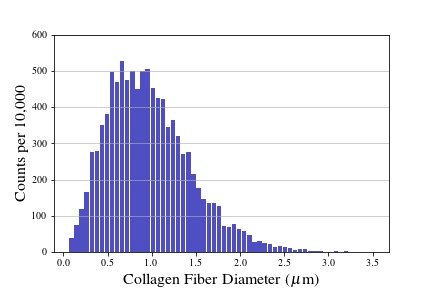
\includegraphics[width=0.45\textwidth]{figures/collagenFiberDiaHistogram.jpg}
    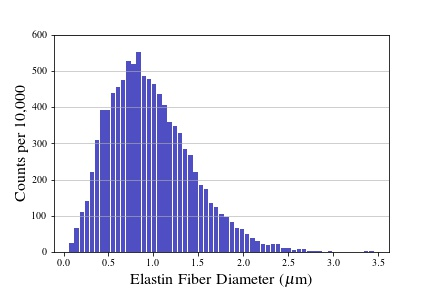
\includegraphics[width=0.45\textwidth]{figures/elastinFiberDiaHistogram.jpg}
    \caption{Typical histograms for collagen and elastin chord diameters pertaining to the statistics reported in Table~\ref{tab:alveolarProp}.  Their tails weigh heavy at the larger diameters, because their distributions are normal in the square root of their diameters.  These histograms are identical, for all practical purposes.}
    \label{fig:septalChordStats}
\end{figure}

The collagen and elastin fibers that make up a septal chord have the same length $L$, they experience the same strain $e$, and they exist at the same temperature $\theta$; therefore, we employ Eqn.~(\ref{Helmholtz1D}) as the governing constitutive equation to describe their mechanical behaviors; specifically, for the collagen fiber in an alveolar chord
\begin{subequations}
    \label{alveolarChord}
    \begin{align}
    \left\{ \begin{matrix} 
    \mathrm{d} \eta^c \\ \mathrm{d} s^c
    \end{matrix} \right\} = \begin{bmatrix}
    C^c / \theta - ( \alpha^c )^2 E^c / \rho^c & \alpha^c E^c / \rho^c \\
    -\alpha^c E^c & E^c
    \end{bmatrix} \left\{ \begin{matrix}
    \mathrm{d} \theta \\ \mathrm{d} e
    \end{matrix} \right\} \\
    \intertext{and for the elastin fiber in an alveolar chord}
    \left\{ \begin{matrix} 
    \mathrm{d} \eta^e \\ \mathrm{d} s^e
    \end{matrix} \right\} = \begin{bmatrix}
    C^e / \theta - ( \alpha^e )^2 E^e / \rho^e & \alpha^e E^e / \rho^e \\
    -\alpha^e E^e & E^e
    \end{bmatrix} \left\{ \begin{matrix}
    \mathrm{d} \theta \\ \mathrm{d} e
    \end{matrix} \right\} 
    \end{align}
\end{subequations}
where $\eta^c$ and $\eta^e$ are the entropy densities (erg/gr.K) for collagen and elastin; $s^c \defeq \lambda F^c / A^c_0$ and $s^e \defeq \lambda F^e / A_0^e$ are the chordal stresses (barye = $\text{dyne/cm}^2$) carried by the collagen and elastin fibers, wherein $\lambda = L/L_0$ is the fiber stretch, $A^c_0$ and $A^e_0$ are their traction-free cross-sectional areas ($\text{cm}^2$), and $F^c$ and $F^e$ are the forces (dyne) they transmit.  Parameters $C^c$ and $C^e$ are their specific heats at constant pressure (erg/gr.K), $\alpha^c$ and $\alpha^e$ are their linear coefficients of thermal expansion (1/K), $E^e$ and $E^e$ are their elastic moduli ($\text{dyne/cm}^2$ = $\text{erg/cm}^3$), and $\rho^c$ and $\rho^e$ are their mass densities ($\text{gr/cm}^3$).  These differential equations are subject to initial conditions considered to be $s^c_0 = s^c |_{L = L_0} = 0$, $s^e_0 = s^e |_{L = L_0} = 0$, $\eta^c = \eta^c_0$ and $\eta^e = \eta^e_0$, where  $\eta_0^c$ and $\eta_0^e$ are their respective entropy densities at rest.

The actual force and entropy of an individual septal chord in our alveolar model is taken to be one third of a fiber's calculated values, as determined by Eqn.~(\ref{alveolarChord}), because each alveolar chord is typically shared between three adjoining alveoli; consequently, 
\begin{equation}
    \label{septalChordCEs}
    F^f = ( A_0^c s^c + A_0^e s^e ) / 3 \lambda 
    \quad \text{and} \quad
    S^f = ( \rho^c V_0^c \eta^c + \rho^e V_0^e \eta^e ) / 3 
\end{equation}  
where $F^f$ (dyne) is a third of the fiber's force carried by a septal chord, and $S^f$ (erg/K) is a third of the fiber's entropy.

Collagen is a fiber comprised of numerous, long, slender, wavy filaments whose waviness, known as crimp, straightens under sufficient deformation \cite{Kastelicetal'78,FreedDoehring05}.  Elastin is a linked fiber network, much like an elastomer, whose filaments between crosslinks rotate to align with an axis of loading under sufficient deformation \cite{AaronGosline81,Urry89}.  Consequently, collagen and elastin both recruit constituent filaments with increasing deformation into an overall, load-bearing, fiber response.  The internal energies of collagen and elastin may therefore be thought of as being comprised of a configurational energy and a strain energy.  As such, both collagen and elastin are modeled as Freed-Rajagopal biologic fibers, which are described in terms of two such internal energies.  Their model is derived from the theory of implicit elasticity in \ref{appImplicitElasticity}.  According to their model, tangent compliances for collagen and elastin are described by
\begin{subequations}
    \label{septalChordModuli}
    \begin{align}
	\frac{1}{E^c (\theta , s^c , e )} & = \frac{e_t^c - e_1^c}{E_1^c e_t^c + 2s^c} + \frac{1}{E_2^c} &
	e_1^c & = e - \alpha^c (\theta - \theta_0) - \frac{s^c}{E_2^c} \\
    \frac{1}{E^e (\theta , s^e , e )} & = \frac{e_t^e - e_1^e}{E_1^e e_t^e + 2s^e} + \frac{1}{E_2^e} &
    e_1^e & = e - \alpha^e (\theta - \theta_0) - \frac{s^e}{E_2^e} 
    \end{align}
\end{subequations}
where $\theta_0$ is body temperature, i.e., 310~K.  Mterial constants $E_1^c$ and $E_2^c$ are the two asymptotic moduli for collagen that bound its response, i.e., $E_1^c \leq E^c \leq E^c_2$, while $E_1^e$ and $E_2^e$ are the two asymptotic moduli for elastin that bound its response, viz., $E^e_1 \leq E^e \leq E^e_2$, both having units of stress (barye = dyne/$\text{cm}^2$), with $e_t^c$ and $e_t^e$ being their respective transition strains, cf.\ \ref{appImplicitElasticity}. 

The material properties needed to model septal chords are listed in Tables~\ref{tab:alveolarProp} \& \ref{tableCollagenElastin}.  From Eqn.~(\ref{thermodynamicConstraints}), these moduli are bound from above by $E^c_{\max} = 4.9 \times 10^9$~barye ($\text{dyne/cm}^2$) and $E^e_{\max} = 1.7 \times 10^9$~barye.  We therefore observe that $E^c_2$ and $E^e_2$ are about 100 times smaller than $E^c_{\max}$ and $E^e_{\max}$.  We recall that temperature $\theta = \theta_0$ in our application, where $\theta_0$ is body temperature, so strains $e^c_1$ and $e^e_1$ defined in the second column above simplify somewhat.  

\begin{table}
    \centering
    \begin{tabular}{|l|l|l|}
        \hline
        \multicolumn{3}{|c|}{Collagen$\vphantom{|^{|^|}}$} \\ \hline
        $\rho^c$ \hfill [$\textrm{gr/cm}^{3^{\phantom{|}}}$] & $1.34$ & 
        Fels \cite{Fels64} \\
        $\eta_0^c$ \hfill [erg/gr.K] & $3.7 \times 10^7$ &  \\
        $C^c$ \hfill [erg/gr.K] & $1.7 \times 10^7$ & 
        Kanagy \cite{Kanagy55} \\
        $\alpha^c$ \hfill [1/C] & $1.8 \times 10^{-4}$ & 
        Weir \cite{Weir48}  \\
        $e^c_t$ & $0.09$ & estimated from TLC $\approx$ 30\% \\
        $E_1^c$ \hfill [barye] & $5.0 \times 10^5$ & authors experience \\
        $E_2^c$ \hfill [barye] & $3.0 \times 10^7$ & authors experience \\ \hline
        \multicolumn{3}{|c|}{Elastin$\vphantom{|^{|^|}}$} \\ \hline 
        Parameter & Value & Reference \\ \hline
        $\rho^e$ \hfill [$\textrm{gr/cm}^{3^{\phantom{|}}}$] & $1.31$ & 
        Lillie \& Gosline \cite{LillieGosline02a} \\
        $\eta_0^e$ \hfill [erg/gr.K] & $3.4 \times 10^7$ & 
        Shadwick \& Gosline \cite{ShadwickGosline85} \\
        $C^e$ \hfill [$\textrm{erg/gr.K}$] & $4.2 \times 10^7$  & 
        Kakivaya \& Hoeve \cite{KakivayaHoeve75} \\
        $\alpha^e$ \hfill [1/C] & $3.2\times 10^{-4}$ & 
        Lillie \& Gosline \cite{LillieGosline02a} \\ 
        $e^e_t$ & 0.4 & Shadwick \& Gosline \cite{ShadwickGosline85} \\
        $E^e_1$ \hfill [barye] & $2.3 \times 10^6$ & Urry \cite[Fig.~18]{Urry89} \\ 
        $E^e_2$ \hfill [barye] & $1.0 \times 10^7$ & 
        Lillie \& Gosline \cite[Fig.~5]{LillieGosline07} \\ \hline
    \end{tabular}
    \caption{Physical properties for hydrated collagen and elastin fibers.  Collagen denatures at around $60^\circ$C \cite{HoermannSchlebusch71}, i.e., above this temperature collagen will shrink rapidly---an effect not modeled here.}
    \label{tableCollagenElastin}
\end{table}

\subsection{Modeling Alveolar Septa Subjected to Shock Waves}
\label{secConjugatePairs}

The thermo\-elastic response of a planar membrane used to model alveolar septa, as described in Eqn.~(\ref{HelmholtzMembraneODEs}), is governed by the following pair of differential equations.  The first set of ODEs establishes the uniform response in Eqn.~(\ref{HelmholtzMembraneODEsUniform}) for a membrane described by
\begin{displaymath}
    \left\{ \begin{matrix}
    \mathrm{d} \eta \\ \mathrm{d} s^{\pi}
    \end{matrix} \right\} = \begin{bmatrix}
    C / \theta - 4 \alpha^2 M / \rho & 
    4 \alpha M / \rho \\
    -4 \alpha M & 4 M
    \end{bmatrix} \left\{ \begin{matrix}
    \mathrm{d} \theta \\ \mathrm{d} \xi
    \end{matrix} \right\} 
\end{displaymath}
while the second set of ODEs establishes the non-uniform response in Eqn.~(\ref{HelmholtzMembraneODEsNonUniformCV}) for a membrane described by
\begin{displaymath}
    \left\{ \begin{matrix}
    \mathrm{d} s^{\sigma} \\ \mathrm{d} s^{\tau}
    \end{matrix} \right\} = \begin{bmatrix}
    4 M / 3 & 0 \\
    0 & G
    \end{bmatrix} \left\{ \begin{matrix}
    \mathrm{d} \varepsilon \\ \mathrm{d} \gamma
    \end{matrix} \right\}
\end{displaymath}
where $s^{\pi} \defeq \pi / h$, $s^{\sigma} \defeq \sigma / h$ and $s^{\tau} \defeq \tau / h$ have units of stress (dyne/$\text{cm}^2$) with $h$ denoting the height or thickness of a spetal membrane that, assuming the volume of a septal membrane remains constant, it is described by $h = h_0 \exp ( -2 \xi )$ where $h_0$ is its traction-free thickness.

From a mechanics perspective, we know a great deal more about alveolar chords than we know about alveolar septa.  More judgment will therefore be required in our construction and parameterization of a material model for alveolar membranes.  

A typical alveolar septum is 4-5 $\mu$m in width \cite{Sukietal11}.  They are comprised of an outside layer of epithelial cells that encase capillaries made of endothelial cells along with a basement membrane that is composed of unorganized collagen and elastin filaments, plus proteoglycans and other extracellular proteins.  This basement membrane, roughly at mid-plane in an alveolar septum, has a width of about $0.5 \, \mu$m \cite{RoanWaters11}.  Inertial forces generated by these membranes are to be based upon a membrane thickness of $\sim\!\!5$~$\mu$m with an approximate density of water, while the structural forces that they carry are to be based upon a basement membrane thickness of $\sim\!\! 0.5$~$\mu$m.  

It is not known how much of the mechanical load is actually carried by the cells in an alveolar septum vs.\ the extracellular basement membrane they encase, but it is generally thought that this basement membrane carries the majority of the load \cite{Sukietal11}.  Therefore, by diminishing the moduli that are appropriate for describing a basement membrane with thickness $\sim\!\! 0.5$~$\mu$m by a factor of 10, we get estimates for effective septal moduli that are applicable when modeling a whole septal membrane with thickness $\sim\!\! 5$~$\mu$m.  We use the model parameters obtained for a visceral pleura membrane \cite{Freedetal17} and the above conjecture to model alveolar septa, as specified in Table~\ref{tableVisceralPleura}.

\begin{table}
    \centering
    \begin{tabular}{|l|l|}
        \hline
        Property & Value \\ \hline
        $\rho$ \hfill [$\textrm{gr/cm}^{3^{\phantom{|}}}$] & $1.1$ \\
        $\eta_0$ \hfill [erg/gr.K] & $5.0 \times 10^6$ \\
        $C$ \hfill [erg/gr.K] & $2.1 \times 10^7$ \\
        $\alpha$ \hfill [1/C] & $1.2 \times 10^{-4}$ \\ \hline
        $\xi_t$ & $0.24$ \\
        $M_1$ \hfill [barye] & $8.0 \times 10^2$ \\
        $M_2$ \hfill [barye] & $2.2 \times 10^5$ \\ \hline
        $\gamma_t$ & $0.4$ \\
        $G_1$ \hfill [barye] & $5.0 \times 10^2$ \\
        $G_2$ \hfill [barye] & $1.5 \times 10^4$ \\ \hline
    \end{tabular}
    \caption{The elastic properties are for visceral pleura taken from \cite{Freedetal17}, divided by 10 to adjust for septal thickness vs.\ basement membrane thickness.  The thermo\-physical properties lie between that of water and collagen, weighted towards that of water and evaluated at body temperature.}
    \label{tableVisceralPleura}
\end{table}

Collagen and elastin appear as thin filaments randomly oriented and somewhat uniformly dispersed throughout a basement membrane, unlike the strongly aligned fibers that appear in septal chords.  Consequently, for our purposes, we model this collective ensemble of tissue and structure types as a homo\-geneous isotropic membrane modeled after the Freed-Rajagopal biologic fiber \cite{FreedRajagopal16} that we have extended to membranes in \ref{appImplicitElasticity}, specifically
\begin{subequations}
    \label{septalCompliances}
    \begin{align}
    \frac{1}{M} & = \frac{\xi_t - \xi_1}{M_1 \xi_t + s^{\pi} / 2} + \frac{1}{M_2} &
    \xi_1 & = \xi - \alpha ( \theta - \theta_0 ) - \frac{s^{\pi}}{4M_2}
    \label{septalDilationCompliance} \\
    \frac{1}{G} & = \Gamma \left( \frac{\gamma_t - 2\varepsilon \gamma - | \gamma_1 |}{G_1 \gamma_t + 2 \varepsilon s^{\tau}} + \frac{1-2\varepsilon}{G_2} \right) & 
    \gamma_1 & = \gamma - \frac{(1 - 2\varepsilon) s^{\tau}}{G_2}
    \label{septalShearCompliance}
    \end{align}
\end{subequations}
where the compliant tangent moduli of $M_1$ and $G_1$ and the stiff, terminal, tangent moduli of $M_2$ and $G_2$ bound their responses in that $M_1 \leq M \leq M_2$ and $G_1 \leq G \leq G_2$, with gradual transitions between their asymptotic bounds being centered around strains of $\xi_t$ and $\gamma_t$.

Finite element technology is used to interpolate the entropy and these stresses, integrated at the Gauss points, to entropies and forces at the vertices of a pentagon, cf.\ Part~\ref{partVariational}.  The actual entropies and forces interpolated to these nodes are halved, because each septal plane belongs to two adjoining alveoli. 

\subsection{Modeling an Alveolar Volume Subjected to Shock Waves}
\label{sec:IdealGasLaw}

Alveoli are connected to bronchial trees via alveolar ducts.  Under normal conditions, air moves in and out of the alveoli via these ducts.  However, when subjected to a stress wave passing over an alveolus, there is no time for the transport of air to take place.  Hence, we can consider the air (and heat) within an alveolus to become `trapped', and the pressure to be uniform therein.  The governing process is therefore adiabatic.  It is under this condition that we model the volumetric response of an alveolar sac.

\subsubsection{Alveoli Filled with Air}

Considering the saturated air within an alveolus to be an ideal gas, then \cite{Davison08}
\begin{equation}
P V = n \! R \theta
\quad \text{or} \quad
\frac{P V}{\theta} = \frac{P_0 V_0}{\theta_0} = n \! R = \mathrm{constant}
\label{idealGas}
\end{equation}
where, in our case, $P_0$ is taken to be atmospheric pressure at sea level (1~bar or $10^5$~Pa or $10^6$~barye), with $V_0$ being that alveolar volume whereat alveolar pressure and plural pressure are both atmospheric, while $\theta_0 = 37^{\circ}$C = 310~K is assigned as body temperature.  Parameter $n$ is the molar content of gas within an alveolus, and $R$ is the universal gas constant.  

The material constants associated with an ideal gas contained within an adiabatic enclosure are
\begin{equation}
\alpha \defeq \frac{1}{L} \left. \frac{\partial L}{\partial \theta} \right|_P =
\frac{1}{3V} \left. \frac{\partial V}{\partial \theta} \right|_P = 
\frac{1}{3\theta_0} \, \frac{P_0 V_0}{P V}
\quad \text{and} \quad
K \defeq -V \left. \frac{\partial P}{\partial V} \right|_{\theta} = 
P_0 \, \frac{V_0 \hspace{0.5pt} \theta}{\theta_0 V}
\label{idealGasConstants}
\end{equation}
with the other two material constants pertaining to moist air at body temperature\footnote{
    The physical properties listed for air were taken from the website \texttt{www.peacesoftware.de} hosted by Berndt Wischnewski.
}
being its mass density $\rho$ of $1.125 \times 10^{-3} \; \text{gr/cm}^3$ and its specific heat $C$ of $1.007 \times 10^7$~erg/gr.K at constant pressure, constrained by the fact that $K < K_{\max} = \rho C / \alpha^2 \theta \approx \rho C \theta$.  An alveolar sac, when modeled as an adiabatic pressure vessel filled with an ideal gas, is described by
\begin{equation}
\left\{ \begin{matrix}
    \mathrm{d} \eta \\ -3 \, \mathrm{d} P
\end{matrix} \right\} = \begin{bmatrix}
    C / \theta - 9 \alpha^2 K / \rho & 
    9 \alpha K / \rho \\
    -9 \alpha K & 9 K
\end{bmatrix} \left\{ \begin{matrix}
    \mathrm{d} \theta \\ \mathrm{d} \Xi
\end{matrix} \right\}
\tag{\ref{Helmholtz3D}}
\end{equation}
where the entropy within an alveolar sac is given by $S^a = \rho V \eta$ whose initial condition is $S^a_0 = \rho V_0 \eta_0$ with $\rho \eta_0$ being the entropy per unit volume of humid air at body temperature and atmospheric pressure, viz., $\rho \eta_0 = 7.770 \times 10^4 \: \text{erg/cm}^3\text{.K}$.  Equation~(\ref{Helmholtz3D}) in conjunction with the physical parameters describing an ideal gas (\ref{idealGasConstants}) result in the following equation governing pressure
\begin{displaymath}
\frac{\mathrm{d} P}{P} = \frac{P_0 V_0 \theta}{P V \theta_0} \left( 
\frac{P_0 V_0 \theta}{P V \theta_0} \, \frac{\mathrm{d} \theta}{\theta} - 
\frac{\mathrm{d} V}{V} \right)
\end{displaymath}
where pressure, volume and temperature all appear as logarithmic rates.

Pressure $P$ is mapped to nodal forces at the vertices of a dodecahedron in our alveolar model.  This requires finite element technology, which is discussed in Part~\ref{partVariational}.

\subsubsection{Alveoli Filled with Fluid}

In lung tissues that are not healthy, fluids may fill alveolar volumes at various regions within a lung, e.g., as could be caused by injury, pneumonia, etc.  In such localities the mechanical response of the local parenchyma will be vastly stiffer than that of healthy tissue, and as such, it will respond very differently to a traveling shock wave.

In the presence of a passing shock wave, we conjecture that an unhealthy alveolar sac, like a healthy one, can be modeled as an adiabatic enclosure, but now the fluid within such an alveolus is considered to behave, momentarily, like an elastic solid.

The thermo\-elastic response of an alveolar volume, as described in Eqn.~(\ref{HelmholtzODEs}), is governed by three sets of uncoupled differential equations.  The first set of ODEs establishes the uniform response of Eqn.~(\ref{HelmholtzODEsUniform}) described by
\begin{displaymath}
\left\{ \begin{matrix}
\mathrm{d} \eta \\ \mathrm{d} \Pi 
\end{matrix} \right\} = \begin{bmatrix}
C / \theta - 3 \alpha^2 K / \rho & 3 \alpha K / \rho \\
-3 \alpha K & 9K
\end{bmatrix} \left\{ \begin{matrix}
\mathrm{d} \theta \\ \mathrm{d} \Xi 
\end{matrix} \right\}
\quad \text{where} \quad
K = K ( \theta , \Pi , \Xi )
\end{displaymath}
with the second set of ODEs in Eqn.~(\ref{HelmholtzODEsSqueeze}) governing the squeeze response
\begin{displaymath}
\left\{ \begin{matrix}
\mathrm{d} \sigma_1 \\ \mathrm{d} \sigma_2
\end{matrix} \right\} = \frac{3}{2} \begin{bmatrix}
2 N_1 & -N_2 \\
-N_1 & 2N_2
\end{bmatrix} \left\{ \begin{matrix}
\mathrm{d} \varepsilon_1 \\ \mathrm{d} \varepsilon_2
\end{matrix} \right\}
\quad \text{where} \quad
\begin{aligned}
N_1 & = N ( \sigma_1 , \varepsilon_1 ) \\
N_2 & = N ( \sigma_2 , \varepsilon_2 )
\end{aligned}
\end{displaymath}
while the third set of ODEs in Eqn.~(\ref{HelmholtzODEsShear}) governs the shear response
\begin{displaymath}
    \left\{ \begin{matrix}
    \mathrm{d} \tau_1 \\ \mathrm{d} \tau_2 \\ \mathrm{d} \tau_3
    \end{matrix} \right\} = \begin{bmatrix}
    G_1 & 0 & 0 \\ 0 & G_2 & 0 \\ 0 & 0 & G_3
    \end{bmatrix} \left\{ \begin{matrix}
    \mathrm{d} \gamma_1 \\ \mathrm{d} \gamma_2 \\ \mathrm{d} \gamma_3
    \end{matrix} \right\}
    \quad \text{where} \quad
    \begin{aligned}
    G_1 & = G ( \tau_1 , \gamma_1 ) \\
    G_2 & = G ( \tau_2 , \gamma_2 ) \\
    G_3 & = G ( \tau_3 , \gamma_3 )
    \end{aligned}
\end{displaymath}
that collectively can be used to describe the thermo\-elastic response of a volume of material.  

How these are to be parameterized will be addressed in next year's work.

\section{Finite Element Implementation of Constitutive Equations}
\label{secFE_CE}

These constitutive models are implemented into our finite element model as hypo-elastic material models \cite{Truesdell55} described by\footnote{
    Constitutive equation $\mathrm{d} \boldsymbol{\sigma} = \mathbf{M} ( \boldsymbol{\sigma}, \boldsymbol{\epsilon} ) \, \mathrm{d} \boldsymbol{\epsilon}$ is that of a hypo-elastic solid \cite{Truesdell55}.  A reasonable visco\-elastic constitutive equation that one could consider would be a Zener \cite{Zener48} solid, which would look something like
    $$ \boldsymbol{\sigma} + \boldsymbol{\tau} \, \mathrm{d} \boldsymbol{\sigma} = \boldsymbol{E}_{\infty} \boldsymbol{\epsilon} + \boldsymbol{\tau} \mathbfsf{E}_0 \, \mathrm{d} \boldsymbol{\epsilon} $$ 
    where $\mathbfsf{E}_{\infty}$ is a matrix of rubbery moduli, $\mathbfsf{E}_0$ is a matrix of glassy moduli, and $\boldsymbol{\tau}$ is a matrix of characteristic relaxation times.  This is a topic for future work.
}
\begin{equation}
\mathrm{d} \boldsymbol{\sigma} = \mathbf{M} ( \boldsymbol{\sigma}, \boldsymbol{\epsilon} ) \, \mathrm{d} \boldsymbol{\epsilon} 
\quad \text{wherein} \quad
\mathrm{d} \boldsymbol{\epsilon} = 
\frac{\mathrm{d} \boldsymbol{\varepsilon} ( \boldsymbol{\lambda} )}
{\mathrm{d} \boldsymbol{\lambda}} \, \mathrm{d} \boldsymbol{\lambda}
\label{hypoelastic}
\end{equation}
where $\boldsymbol{\sigma}$, $\boldsymbol{\epsilon}$ and $\boldsymbol{\lambda}$ are arrays of stress, strain and stretch attributes, respectively, with matrix $\mathbf{M} ( \boldsymbol{\sigma}, \boldsymbol{\epsilon} )$ containing the constitutive tangent moduli, i.e., $\mathrm{d} \boldsymbol{\sigma} / \mathrm{d} \boldsymbol{\epsilon}$, that, in general, may depend upon both stress $\boldsymbol{\sigma}$ and strain $\boldsymbol{\epsilon}$, while strain depends solely upon stretch $\boldsymbol{\lambda}$.

The two-step PECE algorithm presented in \S\ref{sec:1stOrderPECE} presumes the following information.  There is an initial condition for the thermo\-dynamic stresses $\boldsymbol{\sigma}_0$.  An initial far-field deformation gradient $\mathbfsf{F}_0$ is also known, from which initial conditions for the thermo\-dynamic stretches $\boldsymbol{\lambda}_0$ and strains $\boldsymbol{\epsilon}_0$ are readily obtained.  All nodes of integration are to be spaced uniformly in time with $h>0$ designating their separation in time.  

A far-field deformation gradient is considered to be known at the end of the first integration step, i.e., $\mathbfsf{F}_1$, from which the thermo\-dynamic stretches $\boldsymbol{\lambda}_1$ and strains $\boldsymbol{\epsilon}_1$ are readily calculated, with differential rates $\mathrm{d} \boldsymbol{\lambda}_0$ and $\mathrm{d} \boldsymbol{\lambda}_1$ coming from finite difference formul\ae, from which $\mathrm{d} \boldsymbol{\epsilon}_0 = [ \mathrm{d} \boldsymbol{\varepsilon} ( \boldsymbol{\lambda}_0 ) / \mathrm{d} \boldsymbol{\lambda}_0 ] \, \mathrm{d} \boldsymbol{\lambda}_0$ and $\mathrm{d} \boldsymbol{\epsilon}_1 = [ \mathrm{d} \boldsymbol{\varepsilon} ( \boldsymbol{\lambda}_1 ) / \mathrm{d} \boldsymbol{\lambda}_1 ] \, \mathrm{d} \boldsymbol{\lambda}_1$ follow.  Consequently, an initial stress rate can be established, i.e., $\mathrm{d} \boldsymbol{\sigma}_0 = \mathbf{M} ( \boldsymbol{\sigma}_0 , \boldsymbol{\epsilon}_0 ) \, \mathrm{d} \boldsymbol{\epsilon}_0$.  With this information, Heun's method (Eqn.~\ref{startUp1stOrderODEs}) can be called upon to integrate Eqn.~(\ref{hypoelastic}) to determine the thermo\-dynamic stresses and their differential rates out to the end of the first integration step, viz., $\boldsymbol{\sigma}_1$ after which one can determine $\mathrm{d} \boldsymbol{\sigma}_1 = \mathbf{M} ( \boldsymbol{\sigma}_1 , \boldsymbol{\epsilon}_1 ) \, \mathrm{d} \boldsymbol{\epsilon}_1$.    

For the next step, and those that follow, the more stable two-step method of Eqn.~(\ref{1stOrderODEs}) can be called upon to advance a solution for the thermo\-dynamic stresses and their differential rates.  What needs to be stored are variables from the previous step, viz., $\boldsymbol{\sigma}_{n-1}$, $\boldsymbol{\lambda}_{n-1}$ and $\mathrm{d} \boldsymbol{\sigma}_{n-1}$, along with like variables from the current step, viz.,  $\boldsymbol{\sigma}_n$, $\boldsymbol{\lambda}_n$ and $\mathrm{d} \boldsymbol{\sigma}_n$.  Then, given a far-field deformation gradient for the next step, i.e., $\mathbfsf{F}_{n+1}$, one can determine $\boldsymbol{\lambda}_{n+1}$ and $\boldsymbol{\epsilon}_{n+1}$ along with the differential rate $\mathrm{d} \boldsymbol{\lambda}_{n+1}$ obtained from finite difference formul\ae, after which $\mathrm{d} \boldsymbol{\epsilon}_{n+1} = [ \mathrm{d} \boldsymbol{\varepsilon} ( \boldsymbol{\lambda}_{n+1} ) / \mathrm{d} \boldsymbol{\lambda}_{n+1} ] \, \mathrm{d} \boldsymbol{\lambda}_{n+1}$ can be established.  With this information, the PECE method (Eqn.~\ref{1stOrderODEs}) can be called upon to integrate Eqn.~(\ref{hypoelastic}) to determine the thermo\-dynamic stresses and their differential rates out to the end of the next integration step, viz., $\boldsymbol{\sigma}_{n+1}$ along with $\mathrm{d} \boldsymbol{\sigma}_{n+1} = \mathbf{M} ( \boldsymbol{\sigma}_{n+1} , \boldsymbol{\epsilon}_{n+1} ) \, \mathrm{d} \boldsymbol{\epsilon}_{n+1}$.

\subsection{1D Formulation}

For any given alveolar chord, we know its reference length $L_0$ and its current length $L$ from which chordal stretch is described by $\lambda \defeq L / L_0$ and its strain is defined as $e \defeq \ln \lambda$ whose differential rate of change is $\mathrm{d} e = L^{-1} \, \mathrm{d} L$; consequently,
\begin{equation}
    \left\{ \begin{matrix}
    \mathrm{d} \theta \\ \mathrm{d} e
    \end{matrix} \right\} = \begin{bmatrix}
    1 & 0 \\ 0 & 1/L
    \end{bmatrix} \left\{ \begin{matrix}
    \mathrm{d} \theta \\ \mathrm{d} L
    \end{matrix} \right\}
\end{equation}
where the matrix establishes $\mathrm{d} \boldsymbol{\varepsilon} ( \boldsymbol{\lambda} ) / \mathrm{d} \boldsymbol{\lambda}$ in Eqn.~(\ref{hypoelastic}) for a chord, with $\mathrm{d} \boldsymbol{\lambda}$ being the vector to the right of this matrix, and $\mathrm{d} \boldsymbol{\varepsilon}$ being the vector on the left-hand side.  Finite difference formul\ae\ are used to quantify $\mathrm{d} \theta$ and $\mathrm{d} L$.

The matrix of tangent moduli $\mathbf{M} ( \boldsymbol{\sigma} , \boldsymbol{\varepsilon} )$ given in Eqn.~(\ref{hypoelastic}) is Eqn.~(\ref{Helmholtz1D}) for the case of a chord, whose elastic modulus is $E(\theta , s , e)$ with stress defined as $s \defeq F/A = \lambda F / A_0$, where $F$ is the force carried by the chord, and where $A_0$ and $A$ are the chordal cross-sectional areas in its reference and current states, respectively.  Here it is assumed that chordal volume is preserved, which is a reasonable assumption for soft biological structures.  The vector being operated on by this matrix of tangent moduli is $\mathrm{d} \boldsymbol{\varepsilon}$ above, with the constitutive equation returning a vector $\mathrm{d} \boldsymbol{\sigma} = \{ \mathrm{d} \eta , \mathrm{d} s \}^{\mathsf{T}}$.  The numerical method presented in \S\ref{sec:1stOrderPECE} can then be called upon to integrate this hypo-elastic constitutive equation for its thermo\-dynamic stresses $\boldsymbol{\sigma}$.  


\subsection{2D Formulation}

Consider an incoming deformation gradient $\mathbfsf{F} = \mathcal{F}_{ij} \, \vec{\mathbfsf{e}}_i \otimes \vec{\mathbfsf{e}}_j$, $i, j = 1, 2$, whose components $\mathcal{F}_{ij}$ are evaluated in a co-ordinate system associated with a membrane whose base vectors $( \vec{\mathbfsf{e}}_1 , \vec{\mathbfsf{e}}_2 )$, cf.\ Fig.~\ref{figPentagonCoord}, have been re-indexed via an orthogonal matrix $\mathbfsf{P}$ according to \S\ref{secRemedy}.  It is in this co-ordinate system that the components of Laplace stretch $\boldsymbol{\mathcal{U}} = \mathcal{U}_{ij} \, \vec{\mathbfsf{e}}_i \otimes \vec{\mathbfsf{e}}_j$ and its inverse $\boldsymbol{\mathcal{U}}^{-1}$ are quantified via
\begin{equation} 
   \boldsymbol{\mathcal{U}} = \begin{bmatrix}
   a & a g \\ 0 & b
   \end{bmatrix} , \quad 
   \boldsymbol{\mathcal{U}}^{-1} = \begin{bmatrix}
   1/a & -g / b \\ 0 & 1/b
   \end{bmatrix}
   \quad \text{with} \quad
   \begin{aligned}
   \mathcal{U}_{11} & = \sqrt{\mathcal{C}_{11}} & \mathcal{U}_{12} & 
   = \mathcal{C}_{12} / \mathcal{U}_{11} \\
   \mathcal{U}_{21} & = 0 & \mathcal{U}_{22} & 
   = \sqrt{\mathcal{C}_{22} - \mathcal{U}_{12}^{\,2}}
   \end{aligned}
\end{equation}
whose physical attributes for stretch are then defined by
\begin{equation}
    a \defeq \mathcal{U}_{11} > 0 , \quad
    b \defeq \mathcal{U}_{22} > 0 , \quad
    g \defeq \frac{\mathcal{U}_{12}}{\mathcal{U}_{11}}
\end{equation}
wherein $\mathbfsf{C} = \mathbfsf{F}^{\mathsf{T}} \mathbfsf{F}$ denotes the right Cauchy-Green deformation tensor $\mathbfsf{C} = \mathcal{C}_{ij} \, \vec{\mathbfsf{e}}_i \otimes \vec{\mathbfsf{e}}_j$ that is affiliated with a membrane whose components $\mathcal{C}_{ij} = \mathcal{F}_{ki} \mathcal{F}_{kj}$ are evaluated in basis $( \vec{\mathbfsf{e}}_1 , \vec{\mathbfsf{e}}_2 )$.

Given a sequence of deformation gradients spaced at uniform time intervals of $h$, one can construct differential rates for the stretch attributes via finite difference formul\ae\ \cite{FreedZamani18}.  Specifically, from the forward difference formula $\dot{\boldsymbol{\mathcal{U}}}_0 = ( \boldsymbol{\mathcal{U}}_1 - \boldsymbol{\mathcal{U}}_0 ) / h + \mathcal{O}(h)$ one finds that
\begin{subequations}
    \begin{align}
    \mathrm{d} a_0 & = \frac{a_1 - a_0}{h} , \quad
    \mathrm{d} b_0 = \frac{b_1 - b_0}{h} , \quad
    \mathrm{d} g_0 = \frac{a_1}{a_0} \left( \frac{g_1 - g_0}{h} \right) \\
\intertext{while from the backward difference formula $\dot{\boldsymbol{\mathcal{U}}}_1 = ( \boldsymbol{\mathcal{U}}_1 - \boldsymbol{\mathcal{U}}_0 ) / h + \mathcal{O}(h)$ one gets}
\mathrm{d} a_1 & = \frac{a_1 - a_0}{h} , \quad
\mathrm{d} b_1 = \frac{b_1 - b_0}{h} , \quad
\mathrm{d} g_1 = \frac{a_0}{a_1} \left( \frac{g_1 - g_0}{h} \right) \\
\intertext{where the finite difference formul\ae\ for states `0' and `1' are first-order accurate.  A second-order accurate, backward, difference formula $\dot{\boldsymbol{\mathcal{U}}}_{n+1} = ( 3 \, \boldsymbol{\mathcal{U}}_{n+1} - 4 \, \boldsymbol{\mathcal{U}}_n + \boldsymbol{\mathcal{U}}_{n-1} ) / 2h + \mathcal{O}(h^2)$, $n = 1, 2, \ldots , N$, can be used for states `2' and onward, from which one determines that}
\mathrm{d}a_{n+1} & = \frac{3a_{n+1} - 3 a_n + a_{n-1}}{2h} \notag \\
\mathrm{d}b_{n+1} & = \frac{3 b_{n+1} - 2 b_n + b_{n-1}}{2h} \\
\mathrm{d}g_{n+1} & = 2 \frac{a_n}{a_{n+1}} \left( \frac{g_{n+1} - g_n}{h} \right) -
\frac{a_{n-1}}{a_{n+1}} \left( \frac{g_{n+1} - g_{n-1}}{2h} \right) . \notag
\end{align}
\end{subequations}
The associated thermo\-dynamic strains and their differential rates at the $n^{\text{th}}$ step are then quantified via
\begin{subequations}
    \begin{align}
    \xi_n & = \ln \left( \sqrt{\frac{a_n}{a_0} \frac{b_n}{b_0}} \right) & 
    \mathrm{d} \xi_n & = \frac{1}{2} \left( \frac{\mathrm{d} a_n}{a_n} + 
    \frac{\mathrm{d} b_n}{b_n} \right) \\
    \varepsilon_n & = \ln \left( \sqrt{\frac{a_n}{a_0} \frac{b_0}{b_n} } \right) & 
    \mathrm{d} \varepsilon_n & = \frac{1}{2} \left( 
    \frac{\mathrm{d} a_n}{a_n} - \frac{\mathrm{d} b_n}{b_n} \right) \\
    \gamma_n & = g_n - g_0 & 
    \mathrm{d} \gamma_n & = \mathrm{d} g_n
    \end{align}
\end{subequations}
where $n = 0 , 1 , 2 , \ldots , N$.  This supposes initial conditions of $\xi_0 = \varepsilon_0 = \gamma_0 = 0$.  Differential rates of the physical attributes relate to differential rates of the thermo\-dynamic variables according to 
\begin{equation}
    \left\{ \begin{matrix}
    \mathrm{d} \theta \\ \mathrm{d} \xi \\
    \mathrm{d} \varepsilon \\ \mathrm{d} \gamma
    \end{matrix} \right\} = \begin{bmatrix}
    1 & 0 & 0 & 0 \\
    0 & 1/2a & 1/2b & 0 \\
    0 & 1/2a & -1/2b & 0 \\
    0 & 0 & 0 & 1
    \end{bmatrix} \left\{ \begin{matrix} 
    \mathrm{d} \theta \\ \mathrm{d} a \\
    \mathrm{d} b \\ \mathrm{d} g
    \end{matrix} \right\}
\end{equation}
where the above matrix establishes $\mathrm{d} \boldsymbol{\varepsilon} ( \boldsymbol{\lambda} ) / \mathrm{d} \boldsymbol{\lambda}$ in Eqn.~(\ref{hypoelastic}) for a membrane, with $\mathrm{d} \boldsymbol{\lambda}$ being the vector to the right of this matrix, and $\mathrm{d} \boldsymbol{\varepsilon}$ being the vector on the left-hand side.

The matrix of tangent moduli $\mathbf{M} ( \boldsymbol{\sigma} , \boldsymbol{\varepsilon} )$ given in Eqn.~(\ref{hypoelastic}) is Eqn.~(\ref{HelmholtzMembraneODEs}) for the case of a membrane, whose moduli are: an areal modulus $M(\theta , \pi , \xi)$, a squeeze modulus $N( \sigma , \varepsilon )$, and a shear modulus $G( \tau , \gamma )$.  The vector being operated on by this matrix of tangent moduli is $\mathrm{d} \boldsymbol{\varepsilon}$ above, with the constitutive equation returning a vector $\mathrm{d} \boldsymbol{\sigma} = \{ \mathrm{d} \eta , \mathrm{d} \pi , \mathrm{d} \sigma , \mathrm{d} \tau \}^{\mathsf{T}}$.  The numerical method presented in \S\ref{sec:1stOrderPECE} can then be called upon to integrate this hypo-elastic constitutive equation for its thermo\-dynamic stresses $\boldsymbol{\sigma}$.  

After this constitutive equation has been integrated, the ensuing thermo\-dynamic stress attributes can be mapped into components $\mathcal{S}_{ij}$ of a stress tensor $\boldsymbol{\mathcal{S}} = \mathcal{S}_{ij} \, \vec{\mathbfsf{e}}_i \otimes \vec{\mathbfsf{e}}_j$, $i, j = 1, 2$, evaluated in the basis $( \vec{\mathbfsf{e}}_1 , \vec{\mathbfsf{e}}_2 )$ of a membrane; specifically,
\begin{equation}
   \left\{ \begin{matrix}
   \eta \\ \mathcal{S}_{11} \\ \mathcal{S}_{22} \\ \mathcal{S}_{12} = \mathcal{S}_{21}
   \end{matrix} \right\} = \begin{bmatrix}
   1 & 0 & 0 & 0 \\
   0 & 1/2 & 1/2 & 0 \\
   0 & 1/2 & -1/2 & 0 \\
   0 & 0 & 0 & b / a
   \end{bmatrix}
   \left\{ \begin{matrix}
   \eta \\ \pi \\ \sigma \\ \tau
   \end{matrix} \right\} .
\end{equation}
These physical stress components $\mathcal{S}_{ij}$ can be pulled back into components $S_{ij}$ belonging to the Lagrangian, second, Piola-Kirchhoff stress $\mathbfsf{S} = S_{ij} \, \vec{\mathbfsf{e}}_i \otimes \vec{\mathbfsf{e}}_j$ or rotated into components $s_{ij}$ belonging to the Eulerian Kirchhoff stress $\mathbfsf{s} = s_{ij} \, \vec{\mathbfsf{e}}_i \otimes \vec{\mathbfsf{e}}_j$ via 
\begin{equation}
    S_{ij} = \mathcal{U}^{-1}_{ik} \mathcal{S}_{k\ell\,} \mathcal{U}^{-1}_{j\ell}
    \quad \text{or} \quad
    s_{ij} = \mathcal{F}_{ik} S_{k\ell} \mathcal{F}_{j\ell} = 
    \mathcal{R}_{ik} \mathcal{S}_{k\ell} \mathcal{R}_{j\ell}
    \label{membraneStresses}
\end{equation}
where $\boldsymbol{\mathcal{R}} = \mathbfsf{F} \hspace{0.5pt} \boldsymbol{\mathcal{U}}^{-1}$ is the Gram rotation that associates with Laplace stretch, viz., $\mathbfsf{F} = \boldsymbol{\mathcal{RU}}$. 

Components $S_{ij}$ belonging to the Lagrangian, second, Piola-Kirchhoff stress $\mathbfsf{S}$ and components $s_{ij}$ belonging to the Eulerian Kirchhoff stress $\boldsymbol{s}$, as established in Eqn.~(\ref{membraneStresses}), are evaluated in a re-indexed co-ordinate system with base vectors $( \vec{\mathbfsf{e}}_1 , \vec{\mathbfsf{e}}_2 )$.  To map these components back into the co-ordinate system of the `user', one must apply the linear transformations
\begin{displaymath}
    P_{ik} S_{k\ell} P_{j\ell}
    \quad \text{and} \quad
    P_{ik} s_{k\ell} P_{j\ell} 
\end{displaymath}
where $\mathbfsf{P}$ is the orthogonal matrix defined in Eqn.~(\ref{membraneRelabling}).

\subsection{3D Formulation}

From an incoming deformation gradient $\mathbfsf{F} = \mathcal{F}_{ij} \, \vec{\mathbfsf{E}}_i \otimes \vec{\mathbfsf{E}}_j$, $i, j = 1, 2, 3$, whose components $\mathcal{F}_{ij}$ are evaluated in a re-indexed co-ordinate system with base vectors $( \vec{\mathbfsf{E}}_1 , \vec{\mathbfsf{E}}_2 , \vec{\mathbfsf{E}}_3 )$, as established in \S\ref{reindexing3D}, it follows that the components for Laplace stretch $\boldsymbol{\mathcal{U}} = \mathcal{U}_{ij} \, \vec{\mathbfsf{E}}_i \otimes \vec{\mathbfsf{E}}_j$ and its inverse $\boldsymbol{\mathcal{U}}^{-1}$ are given by
\begin{equation}
\boldsymbol{\mathcal{U}} = 
\begin{bmatrix}
a & a \gamma & a \beta \\ 0 & b & b \alpha \\ 0 & 0 & c
\end{bmatrix} 
\quad \text{and} \quad
\boldsymbol{\mathcal{U}}^{-1} = \begin{bmatrix}
1/a & -\gamma / b & -( \beta - \alpha \gamma ) / c \\
0 & 1 / b & -\alpha / c \\
0 & 0 & 1/c
\end{bmatrix}
\label{LaplaceStretch}
\end{equation}
where components $\mathcal{U}_{ij}$ are evaluated according to formul\ae\
\begin{equation}
\begin{aligned}
\mathcal{U}_{11} & = \sqrt{\mathcal{C}_{11}} & 
\mathcal{U}_{12} & = \mathcal{C}_{12} / \, \mathcal{U}_{11} &
\mathcal{U}_{13} & = \mathcal{C}_{13} / \, \mathcal{U}_{11} \\
\mathcal{U}_{21} & = 0 &
\mathcal{U}_{22} & = \sqrt{\mathcal{C}_{22} - \mathcal{U}_{12}^{\,2}} &
\mathcal{U}_{23} & = \bigl( \mathcal{C}_{23} - \mathcal{U}_{12\,} \mathcal{U}_{13} \bigr) / \, \mathcal{U}_{22} \\
\mathcal{U}_{31} & = 0 &
\mathcal{U}_{32} & = 0 & 
\mathcal{U}_{33} & = \sqrt{ \mathcal{C}_{33} - \mathcal{U}_{13}^{\,2} - \mathcal{U}_{23}^{\,2}}
\end{aligned}
\label{LagrangianLaplaceStretch}
\end{equation}
thereby permitting their physical attributes for stretch to be established as
\begin{equation}
a \defeq \mathcal{U}_{11} > 0 , \quad
b \defeq \mathcal{U}_{22} > 0 , \quad
c \defeq \mathcal{U}_{33} > 0 , \quad
\alpha \defeq \frac{\mathcal{U}_{23}}{\mathcal{U}_{22}} , \quad
\beta \defeq \frac{\mathcal{U}_{13}}{\mathcal{U}_{11}} , \quad
\gamma \defeq \frac{\mathcal{U}_{12}}{\mathcal{U}_{11}}
\label{LagrangianPhysicalAttributes}
\end{equation}
wherein $\mathbfsf{C} = \mathbfsf{F}^{\mathsf{T}} \mathbfsf{F} = \mathcal{C}_{ij} \, \vec{\mathbfsf{E}}_i \otimes \vec{\mathbfsf{E}}_j$ is the right Cauchy-Green deformation tensor with components $\mathcal{C}_{ij} = \mathcal{F}_{ki} \mathcal{F}_{{kj}}$.  The stretch attributes $a$, $b$ and $c$ are elongation ratios, while the remaining stretch attributes $\alpha$, $\beta$ and $\gamma$ are the magnitudes of shear, cf.\ \S\ref{secQR3D}. 

Given a sequence of deformation gradients spaced at uniform time intervals of $h$, one can construct differential rates for the stretch attributes via finite difference formul\ae\ \cite{FreedZamani18}.  Specifically, from the forward difference formula $\dot{\boldsymbol{\mathcal{U}}}_0 = ( \boldsymbol{\mathcal{U}}_1 - \boldsymbol{\mathcal{U}}_0 ) / h + \mathcal{O}(h)$ one finds that
\begin{subequations}
\begin{align}
\mathrm{d} a_0 & = \frac {a_1 - a_0}{h} \qquad\qquad
\mathrm{d} \alpha_0 
= \frac{b_1}{b_0} \left(\frac{\alpha_1 - \alpha_0}{h} \right) \notag \\
\mathrm{d} b_0 & = \frac {b_1 - b_0}{h} \qquad\qquad
\mathrm{d} \beta_0 
= \frac{a_1}{a_0} \left( \frac{\beta_1 - \beta_0}{h} \right) 
\label{forwardDifference1stOrder} \\
\mathrm{d} c_0 & = \frac {c_1 - c_0}{h} \qquad\qquad 
\mathrm{d} \gamma_0 
= \frac{a_1}{a_0} \left( \frac{\gamma_1 - \gamma_0}{h} \right) \notag \\
\intertext{while from the backward difference formula $\dot{\boldsymbol{\mathcal{U}}}_1 = ( \boldsymbol{\mathcal{U}}_1 -  \boldsymbol{\mathcal{U}}_0 ) / h + \mathcal{O}(h)$ one gets}
\mathrm{d} a_1 & = \frac {a_1 - a_0}{h} \qquad\qquad
\mathrm{d} \alpha_1
= \frac {b_0}{b_1} \left( \frac{\alpha_1 - \alpha_0}{h} \right) \notag \\
\mathrm{d} b_1 & = \frac {b_1 - b_0}{h} \qquad\qquad
\mathrm{d} \beta_1 
= \frac {a_0} {a_1} \left( \frac{\beta_1 - \beta_0}{h} \right) 
\label{backwardDifference1stOrder} \\
\mathrm{d} c_1 & = \frac {c_1 - c_0}{h} \qquad\qquad 
\mathrm{d} \gamma_1 
= \frac{a_0}{a_1} \left(\frac{\gamma_1 - \gamma_0}{h} \right) \notag \\
\intertext{where the finite difference formul\ae\ for states `0' and `1' are first-order accurate.  A second-order accurate, backward difference formula  $\dot{\boldsymbol{\mathcal{U}}}_{n+1} = ( 3 \, \boldsymbol{\mathcal{U}}_{n+1} -  4 \, \boldsymbol{\mathcal{U}}_{n} + \boldsymbol{\mathcal{U}}_{n-1} ) / 2h + \mathcal{O}(h^2)$, $n = 1, 2, \ldots, N$, can be used for states '2' and onward, from which one determines that}
\mathrm{d} a_{n+1} & = \frac {3a_{n+1} - 4a_{n} +  a_{n-1}}{2h} \notag \\ 
\mathrm{d} b_{n+1} & = \frac {3b_{n+1} - 4b_{n} +  b_{n-1}}{2h} \notag \\
\mathrm{d} c_{n+1} & = \frac {3c_{n+1} - 4c_{n} +  c_{n-1}}{2h} \notag \\
\mathrm{d} \alpha_{n+1} & 
= \frac{2b_{n}} {b_{n+1}} \left( \frac{\alpha_{n+1} - \alpha_{n}}{h} \right) - \frac{b_{n-1}} {b_{n+1}} \left( \frac{\alpha_{n+1} - \alpha_{n-1}}{2h} \right)
\label{backwardDifference2ndOrder} \\
\mathrm{d} \beta_{n+1} & 
= \frac{2a_{n}}{a_{n+1}} \left( \frac{\beta_{n+1} - \beta_{n} }{h} \right) - \frac{a_{n-1}} {a_{n+1}} \left( \frac{\beta_{n+1} - \beta_{n-1}}{2h} \right) \notag \\ 
\mathrm{d} \gamma_{n+1} & 
= \frac{2a_{n}} {a_{n+1}} \left(\frac{\gamma_{n+1} - \gamma_{n}}{h} \right) - \frac{a_{n-1}}{a_{n+1}} \left( \frac{\gamma_{n+1} - \gamma_{n-1}}{2h} \right) . \notag
\end{align}
\end{subequations}
The associated thermo\-dynamic strains and their differential rates at the $n^{\text{th}}$ step have an uniform contribution of
\begin{subequations}
    \label{thermodynamicStrains}
    \begin{align}
    \Xi_n & = \ln \left( \sqrt[3]{\frac{a_n}{a_0} \frac{b_n}{b_0} \frac{c_n}{c_0}} \right) & 
    \mathrm{d} \Xi_n & = \frac{1}{3} \left( \frac{\mathrm{d} a_n}{a_n} + 
    \frac{\mathrm{d} b_n}{b_n} + \frac{\mathrm{d} c_n}{c_n} \right) \\
    \intertext{have squeeze contributions of}
    \varepsilon_{1n} & = \ln \left( \sqrt[3]{\frac{a_n}{a_0} \frac{b_0}{b_n}} \right) & 
    \mathrm{d} \varepsilon_{1n} & = \frac{1}{3} \left( \frac{\mathrm{d} a_n}{a_n} - 
    \frac{\mathrm{d} b_n}{b_n} \right) \\
    \varepsilon_{2n} & = \ln \left( \sqrt[3]{\frac{b_n}{b_0} \frac{c_0}{c_n}} \right) & 
    \mathrm{d} \varepsilon_{2n} & = \frac{1}{3} \left( \frac{\mathrm{d} b_n}{b_n} -
    \frac{\mathrm{d} c_n}{c_n} \right) \\
    \intertext{and have shear contributions of}
    \gamma_{1n} & = \alpha_n - \alpha_0 &
    \mathrm{d} \gamma_{1n} & = \mathrm{d} \alpha_n \\
    \gamma_{2n} & = \beta_n - \beta_0 &
    \mathrm{d} \gamma_{2n} & = \mathrm{d} \beta_n \\
    \gamma_{3n} & = \gamma_n - \gamma_0 &
    \mathrm{d} \gamma_{3n} & = \mathrm{d} \gamma_n
    \end{align}
\end{subequations}
where $n = 0, 1, 2, \ldots, N$.  These suppose initial conditions of $\Xi_{\,0} = \varepsilon_{1\,0} = \varepsilon_{2\,0} = \gamma_{1\,0} = \gamma_{2\,0} = \gamma_{3\,0} = 0$. Differential rates of the physical attributes relate to differential rates of the thermo\-dynamic variables according to
\begin{equation}
    \left\{ \begin{matrix}
    \mathrm{d} \theta \\ \mathrm{d} \Xi \\ \mathrm{d} \varepsilon_1 \\
    \mathrm{d} \varepsilon_2 \\ \mathrm{d} \gamma_1 \\ \mathrm{d} \gamma_2 \\
    \mathrm{d} \gamma_3
    \end{matrix} \right\} = \begin{bmatrix}
    1 & 0 & 0 & 0 & 0 & 0 & 0 \\
    0 & 1/3a & 1/3b & 1/3c & 0 & 0 & 0 \\
    0 & 1/3a & -1/3b & 0 & 0 & 0 & 0 \\
    0 & 0 & 1/3b & -1/3c & 0 & 0 & 0 \\
    0 & 0 & 0 & 0 & 1 & 0 & 0 \\
    0 & 0 & 0 & 0 & 0 & 1 & 0 \\
    0 & 0 & 0 & 0 & 0 & 0 & 1
    \end{bmatrix} \left\{ \begin{matrix}
    \mathrm{d} \theta \\ \mathrm{d} a \\ \mathrm{d} b \\ \mathrm{d} c \\
    \mathrm{d} \alpha \\ \mathrm{d} \beta \\ \mathrm{d} \gamma
    \end{matrix} \right\}
\end{equation}
where the above matrix establishes $\mathrm{d} \boldsymbol{\varepsilon} ( \boldsymbol{\lambda} ) / \mathrm{d} \boldsymbol{\lambda}$ in Eqn.~(\ref{hypoelastic}), with $\mathrm{d} \boldsymbol{\lambda}$ being the vector at the right of this matrix, and $\mathrm{d} \boldsymbol{\varepsilon}$ being the vector on the left-hand side. 

The matrix of tangent moduli $\mathbf{M} ( \boldsymbol{\sigma} , \boldsymbol{\varepsilon} )$ given in Eqn.~(\ref{hypoelastic}) is Eqn.~(\ref{HelmholtzODEs}) for the general case, whose moduli are: an bulk modulus $K(\theta , \Pi , \Xi)$, two squeeze moduli $N_1 = N ( \sigma_1 , \varepsilon_1 )$ and $N_2 = N ( \sigma_2 , \varepsilon_2 )$, and three shear moduli $G_1 = G ( \tau_1 , \gamma_1 )$, $G_2 = G ( \tau_2 , \gamma_2 )$ and $G_3 = G ( \tau_3 , \gamma_3 )$.  The vector being operated on by this matrix of tangent moduli is $\mathrm{d} \boldsymbol{\varepsilon}$ above, with the constitutive equation returning a vector $\mathrm{d} \boldsymbol{\sigma} = \{ \mathrm{d} \eta , \mathrm{d} \Pi , \mathrm{d} \sigma_1 , \mathrm{d} \sigma_2 , \mathrm{d} \tau_1 , \mathrm{d} \tau_2 , \mathrm{d} \tau_3 \}^{\mathsf{T}}$.  The numerical method presented in \S\ref{sec:1stOrderPECE} can be called upon to integrate this hypo-elastic constitutive equation.  

After this constitutive equation has been integrated, the ensuing thermo\-dynamic stress attributes can be mapped into components $\mathcal{S}_{ij}$ of a physical stress tensor $\boldsymbol{\mathcal{S}} = \mathcal{S}_{ij} \, \vec{\mathbfsf{E}}_i \otimes \vec{\mathbfsf{E}}_j$, $i, j = 1, 2, 3$, evaluated in the re-indexed basis $( \vec{\mathbfsf{E}}_1 , \vec{\mathbfsf{E}}_2 , \vec{\mathbfsf{E}}_3 )$ of our dodecahedron; specifically,
\begin{equation}
\left\{ \begin{matrix}
\eta \\ \mathcal{S}_{11} \\ \mathcal{S}_{22} \\ \mathcal{S}_{33} \\
\mathcal{S}_{23} = \mathcal{S}_{32} \\
\mathcal{S}_{13} = \mathcal{S}_{31} \\
\mathcal{S}_{12} = \mathcal{S}_{21}
\end{matrix} \right\} = \begin{bmatrix}
1 & 0 & 0 & 0 & 0 & 0 & 0 \\
0 & 1/3 & 2/3 & 1/3 & 0 & 0 & 0 \\
0 & 1/3 & -1/3 & 1/3 & 0 & 0 & 0 \\
0 & 1/3 & -1/3 & -2/3 & 0 & 0 & 0 \\
0 & 0 & 0 & 0 & c/b & 0 & 0 \\
0 & 0 & 0 & 0 & 0 & c/a & 0 \\
0 & 0 & 0 & 0 & 0 & \alpha b/a & b/a
\end{bmatrix}
\left\{ \begin{matrix}
\eta \\ \Pi \\ \sigma_1 \\ \sigma_2 \\ \tau_1 \\ \tau_2 \\ \tau_3
\end{matrix} \right\} .
\end{equation}
These physical components $\mathcal{S}_{ij}$ can be pulled back into components $S_{ij}$ belonging to the Lagrangian, second, Piola-Kirchhoff stress $\mathbfsf{S} = S_{ij} \, \vec{\mathbfsf{E}}_i \otimes \vec{\mathbfsf{E}}_j$ or rotated into components $s_{ij}$ belonging to the Eulerian Kirchhoff stress $\mathbfsf{s} = s_{ij} \, \vec{\mathbfsf{E}}_i \otimes \vec{\mathbfsf{E}}_j$ via 
\begin{equation}
S_{ij} = \mathcal{U}^{-1}_{ik} \mathcal{S}_{k\ell\,} \mathcal{U}^{-1}_{j\ell}
\quad \text{or} \quad
s_{ij} = \mathcal{F}_{ik} S_{k\ell} \mathcal{F}_{j\ell} = 
\mathcal{R}_{ik} \mathcal{S}_{k\ell} \mathcal{R}_{j\ell}
\end{equation}
where $\boldsymbol{\mathcal{R}} = \mathbfsf{F} \hspace{0.5pt} \boldsymbol{\mathcal{U}}^{-1}$ is the Gram rotation that associates with Laplace stretch, viz., $\mathbfsf{F} = \boldsymbol{\mathcal{RU}}$.

Components $S_{ij}$ belonging to the Lagrangian, second, Piola-Kircchoff stress $\mathbfsf{S}$ and components $s_{ij}$ belonging to the Eulerian Kirchhoff stress $\boldsymbol{s}$, as established in Eqn.~(\ref{membraneStresses}), are evaluated in a re-indexed co-ordinate system with base vectors $( \vec{\mathbfsf{E}}_1 , \vec{\mathbfsf{E}}_2 , \vec{\mathbfsf{E}}_3 )$.  To map these components back into the co-ordinate system of the `user' one must apply the linear transformations
\begin{displaymath}
P_{ik} S_{k\ell} P_{j\ell}
\quad \text{and} \quad
P_{ik} s_{k\ell} P_{j\ell} 
\end{displaymath}
where $\mathbfsf{P}$ is the orthogonal matrix defined in \S\ref{reindexing3D}.

\section{Code Verification and Constitutive Parameterization}
\label{secCE_verifyCode}

All material parameters are assigned from their respective statistical distributions.  For example, there are thirty chords in a dodecahedron comprised of collagen and elastin fibers that are loaded in parallel.  Figure~\ref{figStressStrainFibers} presents a typical set of stress\slash strain response curves for the chords of a dodecahedron whose parameters are displayed in Table~\ref{tabStressStrainFibers}.

\begin{figure}
    \centering
    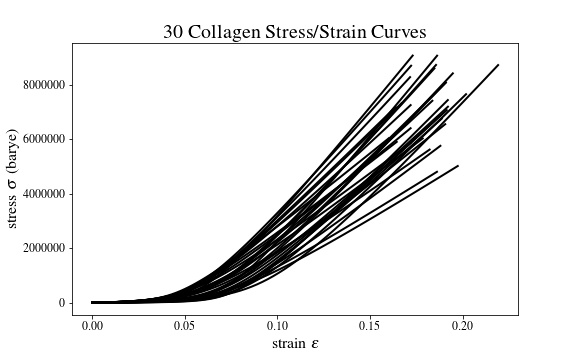
\includegraphics[width=0.45\textwidth]{figures/collagenStressStrain.jpg}
    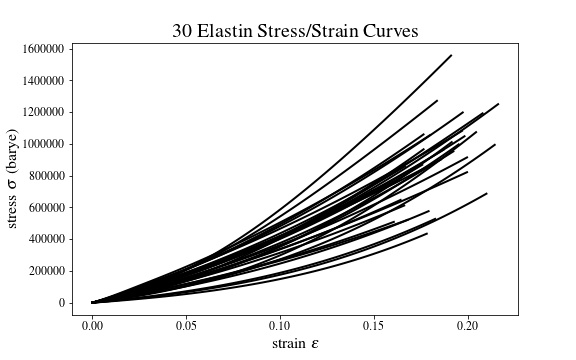
\includegraphics[width=0.45\textwidth]{figures/elastinStressStrain.jpg}
    \caption{Typical stress\slash strain curves for collagen (left) and elastin (right) fibers that make up a septal chord.  Their material parameters have been assigned via statistical distributions.}
    \label{figStressStrainFibers}
\end{figure}

\begin{table}
    \centering
    \begin{tabular}{|l|l|l|l|}
        \hline
        \multicolumn{2}{|c|}{Collagen$\vphantom{|^{|^|}}$} & 
        \multicolumn{2}{|c|}{Elastin} \\ \hline
        $E_1^c$ \hfill [barye] & $5.0 \times 10^{5^{\vphantom{|}}} \pm 2.0 \times 10^5$ &  
        $E_1^e$ \hfill [barye] & $2.3 \times 10^6 \pm 1.0 \times 10^6$ \\
        $E_2^c$ \hfill [barye] & $5.0 \times 10^7 \pm 1.0 \times 10^7$ &  
        $E_2^e$ \hfill [barye] & $1.0 \times 10^7 \pm 2.0 \times 10^6$ \\
        $e^c_t$ & $0.09 \pm 0.015$ &
        $e^e_t$ & $0.4 \pm 0.1$ \\ 
        \hline
    \end{tabular}
    \caption{Physical properties for hydrated collagen and elastin fibers when described with the fiber model of Freed \& Rajagopal \cite{FreedRajagopal16}.}
    \label{tabStressStrainFibers}
\end{table}

Recently, Birzle \textit{et~al}.\ \cite{Birzleetal19} performed experiments on thin slices of rat parenchyma loaded in tension where they removed the collagen and\slash or elastin fiber through collagenase and elastase baths to study their individual behaviors and their interactions under load.
